%       File: VTthesis_template.tex
%     Created: Thu Mar 24 11:00 AM 2016 EDT
%     Last Change: 04/19/2021
%     Author: Chandler Jearls, VT
%
% This template is designed to operate with XeLaTeX.
%
% All elements in the Title, Abstract, and Keywords MUST be formatted as text and NOT as math.
%
%Further instructions for using this template are embedded in the document. Additionally, there are comments at the end of the file that give suggestions on writing your thesis.  
%
%In addition to the standard formatting options, the following options are defined for the VTthesis class: proposal, prelim, doublespace, draft. 

% \documentclass[doublespace,draft,nopageskip]{VTthesis} % nopageskip - Removes arbitrary blank pages.
% This turns off draft mode
\documentclass[doublespace,nopageskip]{VTthesis}

% Using the following header instead will create a draft copy of your thesis
% \documentclass[doublespace,draft]{VTthesis}

% Title of your thesis
\title{Open-Source Parameterized Low-Latency Aggressive Hardware Compressors and Decompressors for Memory Compression}

% You should include 3-5 keywords, separated by commas
\keywords{compression, decompression, accelerator, hardware, parameterized, low-latency}

% Your name, including middle initial(s)
\author{James C. Jearls}

% Change this to your program, e.g. Physics, Civil Engineering, etc.
\program{Computer Engineering} 

% Change this to your degree, e.g. Master of Science, Master of Art, etc.
\degree{Master of Science} 

% This should be your defense date:
\submitdate{May 11, 2021} 

% Committee members. Only have five readers and one chair available.
% Only use the ones you need and don't include the ones you don't need.
% You can also declare a Co-advisor. If you do, the principal and co-advisors
% will be listed as co-advisors on the title page.  Per the VT ETD standards, 
% you should not include titles or educational qualifications such as PhD or Dr.
% You should, however, include middle initials if possible.
\principaladvisor{Ali R. Butt}
\coadvisor{Xun Jian}
\firstreader{Kirk W. Cameron}
\secondreader{Changwoo Min}


% The dedication and acknowledgement pages are optional. Comment them out to remove them.
\dedication{For Alfie, the smartest, happiest dog a man could ask for}
% TODO: add an acknowledgement thanking Dr. Jian's NSF CCF-1919113 grant.
\acknowledge{I would like to thank my lovely wife, Emilie, for her support while I performed this research. I would also like to thank my family and friends for their support. I would like to thank Dr. Jian for his close work on my thesis. I would like to thank Dr. Cameron for mentoring me and guiding me through both my undergraduate and graduate research careers. I would like to thank Dr. Butt for his helpful questions that led me to think more deeply about the topics I was investigating. And I would like to thank Dr. Min for his helpful information on modern memory management algorithms. Finally, I would like to thank the NSF projects 1850025, 1919113, 1942590, 1838271, 1565314, 1939076, each of which have supported me through various points in my academic career.}

% The abstract is required.
\abstract{In recent years, memory has shown to be a constraining factor in many workloads. Memory is an expensive necessity in many situations, from embedded devices with a few kilobytes of SRAM to warehouse-scale computers with thousands of terabytes of DRAM. Memory compression has existed in all major operating systems for many years. However, while faster than swapping to a disk, memory decompression adds latency to data read operations. Companies and research groups have investigated hardware compression to mitigate these problems. Still, open-source low-latency hardware compressors and decompressors do not exist; as such, every group that studies hardware compression is forced to implement it. Importantly, because the devices that can benefit from memory compression vary so widely, there is no single solution to address all devices' area, latency, power, and bandwidth requirements. This work intends to address the many issues with hardware compressors and decompressors. This work implements hardware accelerators for three popular compression algorithms; LZ77, LZW, and Huffman encoding. Each implementation includes a compressor and decompressor, and all designs are entirely parameterized. There are a total of 22 parameters between the designs in this work. All of the designs are open-source under a permissive license. Finally, configurations of the work can achieve decompression latencies under 500 nanoseconds, much closer than existing works to the 263.84 nanoseconds required to read an uncompressed 4 KB page. The configurations of this work accomplish this while still achieving compression ratios comparable to software compression algorithms.} 

% The general audience abstract is required. There are currently no word limits.
%You are also required as of Spring 2016 to include a general audience abstract. This should be geared towards individuals outside of your field that may be reading seeking information about your work. You should avoid language that is particular to your field and clearly define any terms that may have special meaning in your discipline.
\abstractgenaud{Computer memory, the fast, temporary storage where programs and data are held, is expensive and limited. Compression allows for data and programs to be held in memory in a smaller format so less space is used. This work implements a hardware design for compression and decompression accelerators to make it faster for the programs using the compressed data to access it. This work includes three hardware compressor and decompressor designs that can be easily modified and are free for anyone to use however they would like.}

\begin{document}
% The following lines set up the front matter of your thesis or dissertation and are required to ensure proper formatting per the VT ETD standards. 
  \frontmatter
  \maketitle
  \tableofcontents

% The list of figures and tables are now optional per the official ETD standards.  Unless you have a very good reason for removing them, you should leave these lists in the document. Comment them out to remove them.
	\listoffigures
	\listoftables
    \printnomenclature %Creates a list of abbreviations. Comment out to remove it. 

% sample text for abbreviations:

ASIC designs are unconfigurable logic designed to accelerate a task.

\nomenclature{ASIC}{Application-Specific Integrated Circuit}

CAMs allow the memory locations of particular bytes or byte sequences to be quickly found.

\nomenclature{CAM}{Content-Addressable Memory}

FPGAs are used to accelerate applications without spending the resources to create an ASIC design, or for purposes where the design constraints may change over time. They are reconfigurable logic elements.

\nomenclature{FPGA}{Field-Programmable Gate Array}

HDLs are used to describe digital logic designs, similar to how C++ code describes a computer program.

\nomenclature{HDL}{Hardware Description Language}

IoT is a class of objects that incorporate computers and electronics to allow them to network with other devices and operate or record data without human input.

\nomenclature{IoT}{Internet of Things}

LZ is a class of compression algorithms based on papers by Abraham Lempel and Jacob Ziv.
 
\nomenclature{LZ}{Lempel-Ziv}
 
LZW is a number of modifications to the 1978 LZ compression algorithm made by Terry Welch.
 
\nomenclature{LZW}{Lempel-Ziv-Welch}

% The following sets up the document for the main part of the thesis or dissertation. Do not comment out or remove this line.
\mainmatter

\chapter{Introduction} \label{ch:introduction}
From small IoT microcontrollers to warehouse-scale computers, memory is a valuable but limited resource in all modern computing devices. Memory compression is a technique that can enable significantly more effective memory usage by representing data in a more compact format. This allows for less physical RAM to be used for a task, and it can improve performance in memory-bound applications by reducing the time spent swapping to a disk. Additionally, RAM requires a constant power draw to refresh its data, so using less physical RAM has the potential to lower power costs.

In cloud and data center configurations, where the maximum available memory is often used for each CPU, memory can be more expensive than the CPUs used. The AMD EPYC 7763, the highest core count CPU currently on the market, costs \$7890 \cite{epyc_price}. This CPU can utilize up to 4 TB of memory \cite{ibm_epyc}. Extrapolating from the price of the cheapest 64 GB RAM module currently available, \$324, 4 TB of RAM would cost \$20736, which is over 2.62x as expensive as the CPU itself \cite{memory_price}.

Software RAM compression has existed for many years to reduce the need for physical memory. It is supported in Linux, Windows 10, and MacOS \cite{linux_memory_compression, windows10_memory_compression, macos_memory_compression}. However, software decompression adds nearly 75 microseconds of latency to memory read operations. Compared to the latency to read an uncompressed page of memory, 263.84 nanoseconds, decompression adds over 280x more latency. This additional latency can have a significant impact on performance. However, this latency can be significantly reduced if compression and decompression are hardware-accelerated.

There are several existing implementations of hardware-accelerated compressors and decompressors, but these are not suitable for memory compression research \cite{ibm,microsoft}. These designs have poor decompression latencies. They are also targetted towards file compression, which could result in lower effective memory available when using them. These designs are also exclusively proprietary and closed-source, so hardware memory compression research requires building entirely new hardware before it can be evaluated.

The closed-source nature of existing works makes it difficult to conduct memory compression research for a number of reasons. Most importantly, because there are no open-source hardware compressors and decompressors capable of state-of-the-art latencies, researchers must spend months, if not years, designing, implementing, testing, debugging, synthesizing, and optimizing the compression hardware before it can be incorporated into a hardware design and used for compression or decompression. This must be done every time memory compression research is to be conducted, adding significant unnecessary development costs to compression projects. By providing open-source tools, this work empowers the architecture research community to generate area, frequency, and power numbers for simulators, FPGA-accelerate simulations to improve the speed of simulation, and even tape-out chips in less time than ever before.

Existing designs are also very specialized. Applications with different requirements will necessitate different hardware implementations. A low-power microcontroller will require a much different compressor and decompressor than a server with hundreds of CPU cores. To address this need, either many hardware compressors and decompressors must be available, or designs should be highly parameterized. Parameterization allows for fast customization and exploration of the design space, and it allows a single hardware generator to fulfill the needs of many different use cases.

This work attempts to address the shortcomings of existing hardware compressors and decompressors for use in operating system memory compression. This work implements and tests three hardware compressor and decompressor pairs. All implementations are open-source under a permissive license, allowing them to be used and modified as needed by any individual, research group, or enterprise. Every aspect of the design is completely parameterized, from the amount of data compressed by the accelerators to the number of bits in a byte, allowing for complete customizability of the design. Area- or power-constrained systems can choose to use individual compressors and decompressors, and high-performance designs can choose to use multiple compressors and decompressor together for higher compression ratios. The compressors and decompressors are also able to be configured with sub-microsecond decompression latency, even while achieving compression ratios that are comparable to those of software implementations. All of these characteristics mean that this work improves the state of the art for hardware-accelerated memory compression.

The compressors and decompressors in this work are capable of several times lower latency than the existing state of the art hardware compression and decompression accelerators. These hardware compressors and decompressors also use an order of magnitude less area than the existing state of the art. Finally, the compressors and decompressors in this work accomplish all of this while being fully configurable and open-source for anyone to use in the future. 

The rest of this document describes this work and compares it to the existing state-of-the-art. Chapter \ref{ch:literature_review} discusses the existing literature relating to memory compression. Chapter \ref{ch:open-source_hardware_solutions} discusses the designs that comprise this work and the methods used to compare it to the existing state of the art. Chapter \ref{ch:results} presents the results of the comparison to existing works. Chapter \ref{ch:discussion} discusses some limitations of this work and identifies potential future projects based on this work. Finally, Chapter \ref{ch:conclusions} concludes with the broader implications of this work.

\chapter{Literature Review} \label{ch:literature_review}
This chapter reviews the relevant literature on hardware compression and decompression accelerators to demonstrate why existing works do not adequately address the needs of the memory compression research community.

\section{Overview}\label{se:lit_rev_overview}
The following sections discuss many related works and their strengths and weaknesses. These related works are all inadequate in at least one of several ways. They each at least are proprietary designs, have high decompression latencies, do not contain matching compressors and decompressors, are not configurable, or are only implemented on FPGAs. Thus, these are all of the problems that this work attempts to address simultaneously.

\section{Compression Algorithms}\label{se:compression_algorithms}
There are two types of compression algorithms: lossy and lossless. Lossy compression algorithms are often able to achieve much higher compression ratios, but lossy compression often changes the data being compressed in some way. For memory compression, which might hold important data, pointers, or programs, the errors of lossy compression are not acceptable. For this reason, lossless compression is the focus of most works in the field of memory compression.
There are two primary types of lossless compression algorithms: those that change the way characters are encoded to save space and those that utilize repeated sequences of characters to save space. This section describes the existing lossless compression algorithms to give context for the hardware compression designs in this work.

% TODO: add information on other compression algorithms, concluding with the algorithms used in my work.

\subsection{Huffman Encoding}\label{ss:huffman_encoding}
This subsection discusses the steps needed to perform Huffman encoding. It also includes an example to demonstrate the steps.

Huffman encoding achieves minimum redundancy of data by giving characters of data variable lengths \cite{huffman}. The lengths of each encoding are determined by how frequently it appears in the data being compressed. Frequently-occurring data are assigned shorter encodings, and infrequently-occurring data are assigned longer encodings. In this way, data can be optimally encoded such that no two characters' representations could be swapped to achieve a shorter encoding result. 

To accomplish this, Huffman encoding arranges all of the unique characters in the data into a binary tree, where each character is a leaf node. This tree is then used to find the most efficient encoding for each character in the data. There are two types of Huffman encoding: static and dynamic.

Static Huffman encoding uses a pre-made Huffman tree to encode the data. This reduces its flexibility, because the static tree will work very well for certain inputs and poorly for others. However, using a pre-made tree removes all of the work required to create a tree, which simplifies and speeds up the algorithm to encode the data.

Dynamic Huffman encoding is done in two passes. In the first pass, the number of occurrences of each data character are counted to determine their relative frequencies. Afterwards, these frequencies are used to construct a binary tree where each data character is a leaf node. The construction of this tree starts from the two least frequent characters. Every time two nodes are combined under a new parent node, the parent node's frequency becomes the sum of the frequencies of its children. This continues until a single root node encompasses the entire tree.

Once the tree is constructed, the lengths and encodings of the characters can be determined. The number of bits used to represent a character is equal to its depth in the tree from the root node. The encoding of each character is determined by the traversal steps required to reach it from the root node. Every left path in the tree concatenates a `0` to the binary encoding of the character, and each right path concatenates a `1` to the binary encoding.

Finally, once each of the leaf nodes has been given an encoding, the second pass can encode the data. For each character of the input data, the second pass looks up its new encoding and outputs this new encoding. This continues until every character of the input has been encoded.

To decode Huffman-encoded data, only the original Huffman tree is needed. Then, the decompressor can simply traverse the Huffman tree for each bit in the encoded data, stopping and starting from the root node every time a leaf is reached. Including the original Huffman tree with the compressed data can have a significant impact on the compression ratio. To combat this impact, most Huffman compression implementations represent the tree in a canonical form. A canonical Huffman tree represents the data as the number of characters of each depth, then lists the characters in order from the lowest depth to the highest depth. Canonical form is one of the most efficient ways of representing the Huffman tree, and it can be several times smaller than an equivalent tree represented in `plain-text` form, listing each character, the length of its encoding, and the encoding itself.

\subsubsection{Example}\label{sss:huffman_example}
For the purposes of demonstration, the string of characters being compressed for Huffman will be:

\[A,A,A,B,A,A,C,B,B,A,A,B,D,A,A,B\]

Without using Huffman encoding, each of these characters could be encoded with only two bits. An example of the encodings that could be used to do this is shown in Table \ref{tab:default_encoding}. Because there are 16 characters in the example, it would require a total of 32 bits to encode this data.

\begin{table}[htb]
	\centering
	\caption{Example Uncompressed Encoding}
	\begin{tabular}{cc}
	    \toprule
	    Character & Binary Encoding\\
	    \midrule
	    A & 00 \\
	    \midrule
	    B & 01 \\
	    \midrule
	    C & 10 \\
	    \midrule
	    D & 11 \\
	    \bottomrule
	\end{tabular}
	\label{tab:default_encoding}
\end{table}

The first step in dynamic huffman encoding is to count and sort the frequency that each character occurs. The result of the character frequency counting step is shown with the frequencies sorted in Table \ref{tab:character_frequency_count}.

\begin{table}[htb]
	\centering
	\caption{Character Frequency Count}
	\begin{tabular}{cc}
	    \toprule
	    Character & Number of Occurrences\\
	    \midrule
	    A & 9 \\
	    \midrule
	    B & 5 \\
	    \midrule
	    C & 1 \\
	    \midrule
	    D & 1 \\
	    \bottomrule
	\end{tabular}
	\label{tab:character_frequency_count}
\end{table}

Once the sorted list of frequencies is complete, the Huffman tree can be built. To build the Huffman binary tree, create a parent node and set its children to be the two least frequent nodes in the list of existing nodes. Remove the two nodes that were set as children from the list of characters remaining, add their summed frequency values as a new parent node to the list, and re-sort the list by frequency. This step is repeated until there is only a single node remaining in the list. This is the root node. Figure \ref{fig:completed_huffman_tree_example} shows a completed Huffman tree.

\begin{figure}[htb]
	\centering
	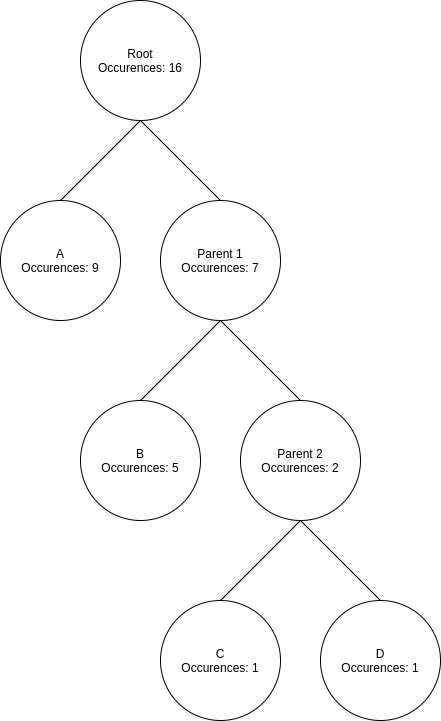
\includegraphics[scale=0.25]{Huffman Tree Example.png}
	\caption{Completed Huffman Tree Example}
	\label{fig:completed_huffman_tree_example}
\end{figure}

Once the Huffman tree is completed, the standard Huffman algorithm is nearly finished. A codeword can be generated for each character in the tree based on its position in the tree. Starting with the root node, the path of each sequence of left and right children reveals the encoding of a character. Each left appends a 0 to the encoding, and each right appends a 1. It is useful to note here that each character's depth in the tree is equal to the number of bits in its encoding. A character encoding based on the tree in Figure \ref{fig:completed_huffman_tree_example} is shown in Table \ref{tab:huffman_encodings}.

\begin{table}[htb]
	\centering
	\caption{Character Encodings}
	\begin{tabular}{ccc}
	    \toprule
	    Character & Character Encoding & Character Encoding Length\\
	    \midrule
	    A & 0 & 1\\
	    \midrule
	    B & 10 & 2\\
	    \midrule
	    C & 110 & 3\\
	    \midrule
	    D & 111 & 3\\
	    \bottomrule
	\end{tabular}
	\label{tab:huffman_encodings}
\end{table}

Now, the only task remaining is to encode each character using the codewords shown in Table \ref{tab:huffman_encodings}. The result of the final character encoding step is shown below. Underscores are used to demonstrate separation between each character for the clarity of the reader. However, it is important to note that delimiters of any kind are unnecessary for Huffman encoding, because every character is a leaf node, so there is no way to mistake the meaning of a sequence of bits.

\[0\_0\_0\_10\_0\_0\_110\_10\_10\_0\_0\_10\_111\_0\_0\_10\]

As can be seen by the above resulting bit sequence, a significant number of bits have been saved. The original encoding would have required 32 bits, but this version only needs 25 bits. This simple example results in a compression ratio ($\frac{initial data size}{compressed data size}$) of 1.28. This simple example is unusually short compared to how Huffman compression would normally be used, so adding the storage overhead from the Huffman tree will remove any compression benefits from Huffman compression. However, for completeness' sake, both a canonical and a plain text Huffman tree example are demonstrated below.

For a canonical Huffman tree, there are many methods of encoding the data. The simple way that is shown here first lists the number of each characters at each depth, then lists each character in order from shallowest to deepest. Because this example uses only four characters, the deepest a leaf node could go in a Huffman tree is a depth of 3. For each depth of the Huffman tree, the number of bits needed to represent the number of characters at that depth is $1+depth$. Because of the Huffman tree can have characters at a depth of up to three, to represent all the depths, the first part of the canonical Huffman tree is as follows: two bits for the number of 1-bit characters, three bits for the number of 2-bit characters, and four bits for the number of 3-bit characters. This sums to a subtotal of nine bits for the depths of the canonical Huffman tree. After the depths, each character is listed. Because the characters can be represented uncompressed as 2-bit values, the character section of the canonical Huffman tree can be anywhere from two to eight bits, depending  on how many characters are in the Huffman tree. Figure \ref{fig:huffman_canonical} below is the binary representation of the canonical Huffman tree of the encodings in Table \ref{tab:huffman_encodings}. Note, this encoding is seventeen bits, while the compressed version of the data only saved seven bits, resulting in an increase in size of ten bits.

\begin{figure}[htb]
	\centering
    \begin{lstlisting}
01_001_0010_00_01_10_11
    \end{lstlisting}
	\caption{Huffman Canonical Tree Example}
	\label{fig:huffman_canonical}
\end{figure}

A plain text Huffman tree is very simple to implement. The most basic method is to represent each character as the number of bits in its encoding, the encoding itself, and the uncompressed character. The current example requires two, three, and two bits for the number of bits, the encoding, and the uncompressed character, respectively. For four characters, that means the plain text form will take up 28 bits, significantly more than the canonical encoding. If the Huffman tree didn't use a character, this can be demonstrated by setting its encoding length value to zero for the plain text representation. Figure \ref{fig:huffman_plain_text} below is the plain text representation of the encodings in Table \ref{tab:huffman_encodings}.

\begin{figure}[htb]
	\centering
    \begin{lstlisting}
01_000_00_10_010_01_11_110_10_11_111_11
    \end{lstlisting}
	\caption{Huffman Plain Text Tree Example}
	\label{fig:huffman_plain_text}
\end{figure}

More details on Huffman encoding and canonical Huffman trees can be found in \cite{huffman, canonicalhuffman}.

\subsection{LZ77}\label{ss:lz77}
While Huffman compression is effective at encoding individual characters, it has limitations that motivate the use of other compression algorithms. Huffman compression with a dynamic tree requires two passes, which requires buffering and the end length to be known for uses like file compression. Additionally, because Huffman only takes advantage of individual characters that occur frequently, it is limited by the size of the Huffman tree and the original size of each symbol. For instance, using 8-bit characters results in a manageable tree size of 256 characters, but the maximum achievable compression ratio is 8x when a character can be represented with a 1-bit code. Using 16-bit characters doubles the maximum achieveable compression ratio to 16x, but increases the size of the Huffman tree to 65,526 characters. Using symbol sizes that are unaligned to the sizes of characters, such as 9- or 10-bit symbols results in poor compression ratios due to misalignment of symbol.

LZ77-based algorithms provide a solution to the shortcomings of Huffman encoding. LZ77-based compression techniques use an algorithm pioneered by Abraham Lempel and Jacob Ziv in 1977 \cite{lz77}. When patterns of characters are repeated in data, LZ77 techniques use references to previous instances of the patterns to represent the data more efficiently. These references are bounded in a sliding window of the most recent data to pass through the compressor. By compressing repeated patterns of characters, maximum compression ratios can be much higher. Additionally, by compressing based on the history of the data, LZ77 avoids needing to send metadata like Huffman does.

For LZ77 compression, a sliding window of a fixed size stores the past history of the compressor. As characters are fed into the compressor, the compressor checks to see if each sequence of characters it receives already exists in the sliding window. If it does, instead of representing the characters as literal characters, it represents them as a pointer-length pair. This pair contains both a pointer to the starting position of a character sequence in the sliding window and the length of the matching character sequence. In this way, even very large sequences of repeated data can be compressed down to only a few bytes.

When LZ77 data is decompressed, the decompressor also keeps track of a sliding window of the data that has been decompressed. Whenever the decompressor is given a pointer-length pair, the decompressor looks up the pointer and reads a number of characters after it equal to the length of the pair. A benefit of this encoding is that it does not require any metadata to be shared between the compressor and decompressor, they both automatically build up identical histories as they process the data.

\subsubsection{Example}\label{sss:lz77_example}
The LZ77 example will use the string shown in Figure \ref{fig:lz77_example_text} to demonstrate the result of LZ77 compression. As with the Huffman example, the characteristics of the example like the compression ratio are not necessarily indicative of the average compression ratio that is achieved by LZ77 on most inputs. However, the example is useful for demonstrating the general format of an LZ77 implementation.

Figure \ref{fig:lz77_compressed_text} shows an example of compressing the example text with LZ77. Each bracketed entry represents a character pattern that has already occurred in the history and that is three characters or longer. Three characters was chosen because this work requires at least three characters in a pattern for the pattern encoding to be less than or equal to the length of the pattern itself. Other variants of LZ77, like LZ4, choose four characters for this cutoff, but the same principles still apply \cite{lz4}.

Each pattern shown in Figure \ref{fig:lz77_compressed_text} follows the form \{pattern starting index, number of characters\}. So, for example, \{3,6\} represents the pattern starting at index three that is six characters long: ` quick`.

\begin{figure}[htb]
	\centering
    \begin{lstlisting}
The quick brown fox jumps over the lazy dog. The brown fox is very quick, and the lazy dog's nap is over.
    \end{lstlisting}
	\caption{LZ77 Example Text}
	\label{fig:lz77_example_text}
\end{figure}

\begin{figure}[htb]
	\centering
    \begin{lstlisting}
The quick brown fox jumps over the lazy dog. {0,4}{10,10}is very{3,6}, and{30,13}'s nap is{24,5}.
    \end{lstlisting}
	\caption{LZ77 Compressed Text}
	\label{fig:lz77_compressed_text}
\end{figure}

\subsection{LZ78 (LZW)}\label{ss:lz78}
LZ78-based compression techniques such as LZW instead use an algorithm published by Lempel and Ziv in 1978, after their first seminal paper on compression \cite{lz78}. Like LZ77, LZ78 works by representing sequences of characters as references, but instead of representing them as pointer-length pairs, LZ78 represents references as dictionary entries. These dictionary entries are built by the compressor and rebuilt by the decompressor as the data is read, so there is no need to transmit a dictionary separately.

LZW is a modification of LZ78 published by Terry Welch in 1984 \cite{lzw}. LZW was developed as a simpler, faster algorithm for compression than existing LZ77 or LZ78 algorithms, but with the goal of still taking advantage of many of the redundancy opportunities that LZ77 and LZ78 take advantage of \cite{lzw}. LZW is able to take advantage of the same character repeated multiple times in a row and of sequences of characters that occur multiple times in the data.

When compressing with LZ78, every sequence of inputs is added to a dictionary. Initially, the dictionary contains as many entries as there are possible unique characters. Then, as data is streamed through the LZ78 compressor, it adds entries to the dictionary. Anytime a sequence of two or more characters is no longer able to be found in the dictionary, it is added to the dictionary, and the sequence of characters starts from the final character in the sequence that caused it to not match any existing entries. This continues for all of the input characters, and then each character output from the dictionary must be the number of bits required to represent the number of entries in the dictionary. This means that as the dictionary gets longer, the length of each output of the compressor also gets larger to allow it to represent all the valid indices in the dictionary. More information and examples of LZW can be found in Welch \cite{lzw}.

\subsection{Deflate}\label{ss:deflate}
Deflate is a combination of LZ77 and Huffman encoding \cite{deflate}. First, LZ77 compression is performed. Next, this result is compressed with Huffman. By combining these two algorithms, Deflate is able to take advantage both of the pattern matching of LZ77 and the improvements in character representation of Huffman encoding. Because it takes advantage of both, its compression ratios are higher than either individually. These high compression ratios make it a good candidate for memory compression.

\section{Existing Hardware Compressors and Decompressors}\label{se:existing_hardware_compressors_and_decompressors}
This section discusses existing hardware accelerators that contain matching compressors and decompressors.

\subsection{Existing Memory Compressors and Decompressors}\label{ss:other_memory_compressors_and_decompressors}
The goals of Compresso are similar to the goals of this work: enabling low-latency memory compression to increase effective memory size \cite{compresso}. However, because Compresso only compresses blocks of 64 bytes, it is only able to achieve compression ratios of 1.85x. This makes it unsuitable for aggressive compression of memory data.

\subsection{Proprietary Compressor-Only Hardware}\label{proprietary_compressor-only_hardware}
This subsection discusses proprietary hardware accelerators that only implement the compressor, relying on software to perform the decompression.

\subsubsection{ASIC Designs}\label{sss:asic_compressor_designs}
Lee et al. verify an LZ4 compressor design in an FPGA, then fabricate it on a 65 nm process node \cite{hardwarelz4}. However, this design is limited to patterns of only 31 bytes, which limits the compression ratios that it can achieve.

\subsubsection{FPGA Designs}\label{sss:fpga_compressor_designs}
Rigler et al. implements separate hardware compressors that use Huffman and LZ77 \cite{fpgahuffmanlz77}. The designs are separate, but the authors claim that it is possible to merge the designs together to implement GZIP. Unlike many designs, the Huffman compressor of this design supports dynamic Huffman encoding, which significantly complicates the hardware.

Abdelfattah et al. use OpenCL to implement GZIP on an Altera FPGA \cite{gziponachip}. This GZIP compressor supports dynamic Huffman encoding and achieves compression ratios over 2x. This design is implemented with high-level synthesis tools, which have a reputation for producing slow, inefficient designs. However, the OpenCL implementation is shown to be very close to a hand-programmed Verilog design in area, speed, and compression ratio.

Luo et al. implement a multi-core GZIP compressor for use with the Hadoop Distributed File System \cite{hdfsgzip}. This work uses static Huffman encoding. The hardware implementation enables a speedup of 70x compared to software compression, which doubles the performance of HDFS.

Identifying that FPGA compressors are limited by CPU-FPGA communication speed, Qiao et al. implement a high-throughput Deflate compression accelerator \cite{fpgadeflate}. Their design uses the extremely high-speed communication of Intel's HARPv2 platform to overcome existing communication bottlenecks for FPGAs. Like many other compressors, they modify the hash table to allow it to work in parallel and use a static Huffman tree to allow Huffman to easily pipeline with the LZ77 compressor.

Ribeiro implements an LZ77 compressor and a static Huffman encoder on an FPGA with a general-purpose CPU that passes data between them and manages them \cite{ribeiro}. The Zynq devices that the design is implemented on is limited to 123 MiB/s by its CPU, and achieves a speedup of 1.5x over the Zynq ARM processor alone.

\subsection{Proprietary Decompressor-Only Hardware}\label{ss:proprietary_decompressor-only_hardware}
The only work relevant work that implements a Deflate decompressor without a matching compressor is done by Ledwon et al. \cite{deflatedecompression}. This work is implemented in C++ and synthesized with Xilinx's high-level synthesis tools. The decompressor is fully Deflate-compliant, so it supports many features that are often deemed unnecessary for hardware compressors or decompressors.

\subsection{Open-Source Hardware Compressors and Decompressors}\label{ss:open-source_hardware_compressors_and_decompressors}
This subsection discusses open-source hardware accelerators that have a matching compressor and decompressor.

\subsubsection{FPGA Designs}\label{sss:open_fpga_designs}
Nunez-yanez created the open-source X-MatchPROvw, implementing the XMatchPro compression algorithm \cite{xmatchpro}. This hardware compressor and decompressor is a dictionary-based pattern compression technique, and the design is capable of four bytes per cycle compression and decompression throughput.

Vijlbrief implements a configurable Deflate compressor and decompressor designed for FPGAs \cite{hdldeflate}. However, this design requires multiple cycles per compressed or decompressed byte, so it is not suitable for low-latency compression and decompression of memory. Additionally, although the HDL-deflate design is partially parameterized, it has many fewer `knobs` for parameterization than this work, as can be seen in Figure \ref{fig:open-source_parameterization_comparison}.

\begin{figure}[htb]
	\centering
	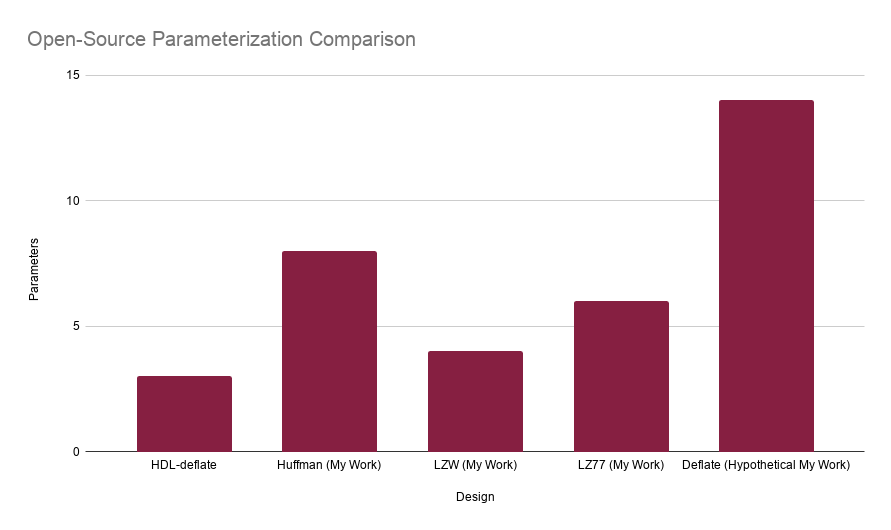
\includegraphics[scale=0.44]{Open-Source Parameterization Comparison.png}
	\caption{Open-Source Parameterization Comparison}
	\label{fig:open-source_parameterization_comparison}
\end{figure}

\subsection{Open-Source Compressor-Only Hardware}\label{ss:open-source_compressor-only_hardware}
This subsection discusses open-source hardware accelerators that only implement the compressor. These rely on a software implementation of the decompression algorithm.
\subsubsection{FPGA Designs}\label{sss:open_fpga_compressor_designs}
Schrittwieser implements a LZRW1 compressor core \cite{lzrw1}. This core requires two cycles per byte and does not have a matching decompressor, so it is not suitable for low-latency compression and decompression of memory.

\subsection{Proprietary Complete Deflate-Like Hardware Compressors and Decompressors}\label{ss:complete_deflate-like_hardware_compressors_and_decompressors}
This subsection discusses proprietary hardware compressors and decompressors that implement Deflate-like algorithms. For the purposes of this discussion, a Deflate-like algorithm is one that uses LZ77 compression followed by Huffman compression.

\subsubsection{ASIC Designs}\label{sss:asic_designs}
IBM has created a Deflate compression and decompression engine that is included in both their POWER9 and z15 processors \cite{ibm}. IBM's implementation is capable of handling data at a rate of 8 bytes/clock, allowing for very high compression and decompression bandwidth \cite{ibm}. The IBM design uses completely accurate near-history CAM and a pseudo-CAM for the older sliding window history to limit CAM area. Additionally, IBM's Huffman encoder builds dynamic trees, unlike many other works that build in a static Huffman encoding to remove the required tree-building process.

The AHA Products Group sells multiple PCIe cards that implement GZIP, which uses Deflate \cite{aha}. While there is not much published information about these cards, they support Deflate, GZIP, ZLIB, and LZS compression, and they scale from 10 Gbps to 80 Gbps compression throughput.

\subsubsection{FPGA Designs}\label{sss:fpga_designs}

Microsoft implements a compressor and decompressor capable of Deflate \cite{microsoft}. The LZ77 compression of this Deflate accelerator is slightly modified to allow LZ77 to be executed in parallel, and the Huffman encoder and decoder uses a static Huffman tree. This design also utilizes over 20 pipeline stages to enable its high clock speeds on an FPGA.

Microsoft also implements its own Xpress9 compression algorithm \cite{xpress9}. Xpress9 is very similar to Deflate, with an LZ77 stage and a Huffman stage. This design is intended to accelerate file compression and decompression in large-scale storage servers. Like Microsoft's other compressor and decompressor, this design processes multiple bytes in parallel to improve the bandwidth of the design. However, unlike Microsoft's Deflate implementation, the Xpress9 design uses a Nios II FPGA soft-core to compute the Huffman encoding. 7 of this design on an FPGA are able to support up to 128 threads of data at 2.4Gbps.


\chapter{Open-Source Motivation}\label{ch:open-source_motivation}
The movement for open-source software has been gaining momentum over the past several decades. Linux is used by most of the internet, the cloud, supercomputers, and even in Android phones and Chromebooks. GCC and LLVM, open-source compiler projects, are widely used. Companies like Amazon, Facebook, Google, Microsoft, and Mozilla are releasing open-source libraries, languages, and tools.

This makes it easy to perform research, because if one is interested in a kernel optimization, they can implement it in the Linux kernel. If one is interested in a virtual memory feature, or a scheduler improvement, or fixing a filesystem bug, these can all be done without building an entire operating system from scratch. In the same way, if one is interested in a compiler optimization, they can implement it in GCC or LLVM without buildling an entire compiler. If one is interested in scientific computing, simulation, animation, or machine learning, there are open-source tools that form a strong starting point so one does not need to create these from nothing every time.

However, until recently, hardware has not enjoyed nearly the same scale of openness and work sharing that software has. As in many hardware domains, there are very few hardware compressors and decompressors that are open-source. This means that, every time a researcher is interested in a new advancement in compression or decompression, they must first implement it in hardware, then test it and debug it. Only when the entire design is working correctly and optimized for area, frequency, and power can the researchers utilize this design for its intended use: compression acceleration. This means potentially months of work, expensive FPGAs for testing or clusters for simulation, and redundant work, often implementing the same algorithms that have already been created many times.

It is clear that there is a need for open-source compression and decompression hardware designs. Existing open-source hardware designs have high latencies, are not very configurable, or are made for a very specific purpose. These designs intend to have low latencies, be extremely configurable, and to be able to be used for many purposes. By open-sourcing this work under the MIT license, anyone will be able to  use it, opening the door for people who are interested in using hardware compressors and decompressors to do so without needing to implement the hardware themselves. By providing designs that have already been implemented and verified, this work has the potential to save thousands of hours of wasted engineering time for those in the field of hardware compression and decompression. In the same way that Linux or GCC are often the default choices for operating system or compiler, it is hoped that this work will become the default choice for hardware compression and decompression.

\chapter{Open-Source Hardware Solutions} \label{ch:open-source_hardware_solutions}
This chapter reviews the contributions of this work. It contains arguments for what makes the work valuable and details about how the work was implemented. It also discusses the high-level design choices and the reasons they were made.

\section{Overview}\label{se:overview}
My work is comprised of three separate pairs of open-source, parameterized compressors and decompressors. The whole work is open-source under the MIT license, so it can be reused. All designs in the work are also entirely parameterized to allow for easy configuration. The first set of compressors and decompressors implements a heavily modified Huffman encoding, the second implements a very slightly modified LZW, and the last implements a modified LZ77.

\subsection{Open-Source}\label{ss:open-source}
As was discussed in Chapter \ref{ch:open-source_motivation}, there is a clear need for more open-source hardware compressor and decompressor designs. This is especially true for low-latency designs. For this reason, all of the designs, scripts, and workflow for this work will be open-sourced under the MIT license. The MIT license gives nearly unlimited freedom to any group or individual to use, modify, or sell the designs in any way they may desire.

In the spirit of open-source, all of the tools used to debug, test, and simulate the work are fully open-source as well. This means that anyone can recreate nearly every aspect of this work for free, without paying for any expensive licenses. The only proprietary software used by this work is the Synopsys Design Compiler, which was used for synthesis of the design to find frequency and area estimates. Although there are currently open-source projects targeting synthesis, they were still in development when this work was started, so they were not considered.

\subsection{Parameterized}\label{ss:parameterized}
Each of the designs in this work are fully parameterized. This means that every aspect of the design is controlled by a parameter. Every single number in the source code of the design is either a configurable parameter or derived from one or more configurable parameters. Even the number of bits in a byte is configurable in this design. This provides a number of benefits.

It is important to note that, unlike with software, fully parameterizing the design is very uncommon in the world of hardware. If hardware is parameterized at all, it is normally limited to a small number of macros that control the sizes of buffers or other structures. \cite{hdldeflate} is a good example of this, as the design does have three parameters, but they only control the sizes of buffers and a search window. The three designs that comprise this work have over 20 parameters in total, and this allows the designs to be configured for frequencies spanning several hundred MHz and areas that are over an order of magnitude different. Not only are the sizes of buffers different between configurations, so are state machine characteristics, numbers and sizes of arithmetic operators, and even the numbers of many modules that are instantiated. This new level of parameterization separates this work from any existing hardware compressors or decompressors.

The first, most important benefit of fully parameterized designs is that the designs are easily configurable. This allows the designs to more easily fit area, frequency, power, and latency constrains without needing to be tweaked. This means that these designs can potentially be used for tiny microcontrollers and massive datacenters without modifying the source code.

Another benefit of the parameterized nature of the designs is the speed of design space exploration. Because everything is parameterized, multiple configurations of the designs can be simultaneously tested for compression ratio, frequency, area, and power. This speeds up the development cycle significantly, reducing the human effort needed to make decisions on design trade-offs.

\subsection{Implementation Language}\label{ss:implementation_language}
This work was initially started in Verilog. However, after a brief trial run switching a module over from Verilog to Chisel, every component of the design was implemented in Chisel. Chisel has a number of benefits over Verilog. Verilog required 2-3x more lines of code on average compared to Chisel. Chisel was significantly faster to write, and it generates well-formatted Verilog, so there are never any issues with synthesizing a Chisel design. Chisel error codes are easy to understand and fix. Most importantly, Chisel language features make it very easy to parameterize the design. Parameterizability was critical for this work, as fast design space exploration was very important to optimizing the hardware.

\subsection{Compressors and Decompressors}\label{ss:compressors_and_decompressors}
The compressors and decompressors included in this work implement variations on popular compression and decompression algorithms. The variations are all made to reduce latency or area and are configurable. The algorithms implemented are Huffman encoding, LZW, and LZ77.

\section{Huffman}\label{ss:huffman}
\subsection{High-Level Design Choices}\label{se:huffman_design_choices}
This section of the paper describes the high-level design of each of the compressors and decompressors, the modifications to the algorithms used, and the motivations for the changes. Information about the low-level implementation details of the design is included in a later section.

\subsubsection{Compressor}\label{sss:huffman_compressor_design}
The Huffman compressor is a fully parameterized hardware compressor implementation. The parameters of the design, along with the typical values chosen for them, are shown in \ref{tab:huffman-configuration-table}. The Huffman compressor supports dynamic Huffman encoding, so instead of simply translating input data with a static lookup table, it performs significant computation on the input data. This allows it to have a higher compression ratio for most workloads than would be possible with a static table.

\begin{table}[htb]
	\centering
	\caption{Configurable Huffman Parameters and their typical values.}
	\begin{tabular}{cc}
	    \toprule
	    Parameter & Typical Value \\
	    \midrule
	    characters to compress & 4096 \\
	    \midrule
	    bits in a character & 8 \\
	    \midrule
	    characters in the Huffman tree & 16 \\
	    \midrule
	    maximum allowed bits in a codeword & 10 \\
	    \midrule
	    character counting frequency parallelism & 8 \\
	    \midrule
	    compressor output encoding parallelism & 8 \\
	    \midrule
	    include statistics on compressed data & false \\
	    \midrule
	    allow for inputs smaller than the `characters to compress` size & false \\
	    \midrule
	    parallel compressor inputs & false \\
	    \midrule
	    parallel compressor outputs & false \\
	    \midrule
	    parallel decompressor inputs & false \\ 
	    \midrule
	    parallel decompressor outputs & false \\
	    \bottomrule
	\end{tabular}
	\label{tab:huffman-configuration-table}
\end{table}

Another benefit of the Huffman compressor design is its modularity. Because Huffman compression requires many different steps, every stage of the process has been separated into its own module. Thanks to this modularity, single components of the design can be modified or replaced without affecting the rest of the design.

The first, most significant difference between this hardware Huffman compressor and a standard implementation is the size of the Huffman tree. This design uses a truncated Huffman tree, meaning only the most frequently occurring characters are used in the Huffman tree that is generated. The number of characters allowed in the Huffman tree is controlled by the `characters in the Huffman tree` parameter. The remainder of the characters are represented with an escape character that is used to signal that a literal character, not character encodings, follow. This escape character adds a small amount of compression overhead, but because it is only used for the least frequently occurring characters, the overhead is not significant in most cases.

Similarly, this compression implementation is able to normalize Huffman trees to a chosen height. While normally, a Huffman tree would have a worst-case depth equal to the number of characters in the tree, this implementation is able to further reduce this worst-case depth to be equal to the `maximum allowed bits in a codeword` parameter. In this way, the amount of hardware can be reduced by limiting the total number of bits of a codeword in the encoding. This normalization has a price. Because there is a limited encoding space, sometimes, there is not room to reduce the depth of a character to the depth desired. In these cases, characters less than this depth are pushed deeper, opening up additional room in the encoding space, until all characters can be represented correctly. This also has a small impact on the compression ratio of the design, because the characters that are moved in the tree to generate more encoding space are still some of the least frequently occurring characters, so slightly lengthening them often does not make much of a difference.

Additionally, most software Huffman compressors represent the Huffman tree in canonical Huffman tree form. This is a special format that reduces the size of the tree. However, this design uses a plain text Huffman tree. In this tree, each character of the tree has its length, its encoding, and the actual character data. A plain text Huffman tree is used for two reasons: first, the design uses fewer characters than most designs, and second, canonical Huffman trees are more complicated to parse than plain text. The first reason means that not using a canonical form for the tree does not affect this design as much as it would affect a design that used usual Huffman algorithm. The second reason means that the decompressor can be significantly faster, because it needs to do much less parsing and computation to determine what the Huffman tree looks like. 

Finally, this Huffman compressor has two configurable options for exploiting parallelism: the character frequency counting and the final character encoding. Both of these can be configured with parameters, allowing the design to be optimized for extreme bandwidth and low-latency or to be optimized for area at the cost of latency and bandwidth.

\subsubsection{Decompressor}\label{sss:huffman_decompressor_design}
Compared to the compressor, the Huffman decompressor is very simple. It uses all of the same parameters as the Huffman compressor. It contains a simple state machine that controls the reading of Huffman tree data into internal lookup tables. Once this is completed, for each parallel encoder in the compressor, there is a parallel decoder that searches for its input data in the internal lookup tables. Each decoder is capable of a steady one byte per clock cycle, so its throughput is nearly perfectly scalable with the compression parallelism.

\subsection{Implementation Details}\label{se:huffman_implementation_details}
This section of the paper describes the low-level implementation details of each of the compressors and decompressors and the reasoning for those implementations.

\begin{figure}[htb]
	\centering
	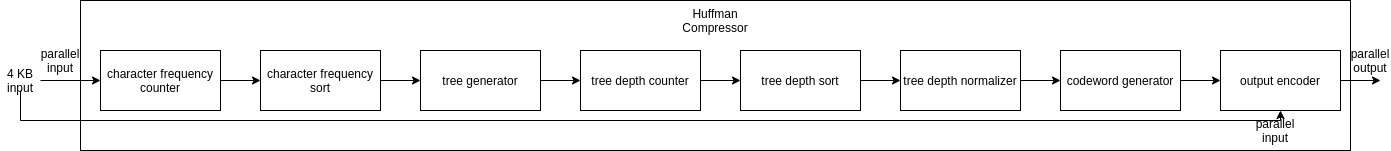
\includegraphics[scale=0.33]{Huffman Compressor Block Diagram.png}
	\caption{Huffman Compressor Block Diagram}
	\label{fig:huffman_compressor_block_diagram}
\end{figure}

\subsubsection{Compressor}\label{sss:huffman_compressor_implementation}
Huffman encoding is the most complicated of the hardware accelerators implemented in this work. The compressor consists of multiple modules (see Figure \ref{fig:huffman_compressor_block_diagram}), each representing one stage of Huffman compressor, all connected with ready/valid interfaces. The design consists of a character frequency counter, a character frequency sort, a tree generator, a tree depth annotation traversal, a sort for the depths of characters in the tree, a character depth normalizer, a codeword generator, and a compressed data output.

The character frequency counter takes as input a number of characters determined by the `character counting frequency parallelism` parameter. This module iterates through the entire input data, counting how many occurrences of each possible character value there are. Once this is complete, it passes an array of the total number of occurrences for each character to the character frequency sort.

The character frequency sort module sorts the frequencies it is given, but requires two passes to perform the sort. The first pass sorts the `characters in the Huffman tree` most frequent characters and sums the number of occurrences of characters that are excluded. Then, so all the characters can be represented in some way, the second pass uses this sum of occurrences for the escape character. The escape character is sorted into the existing character data, then the characters and their frequencies are passed to the tree generator. The end of this module matches up with the state of the compression example shown in Table \ref{tab:character_frequency_count}, but with the addition of the escape character. 

The tree generator builds a Huffman tree with hardware registers that can be configured as pointers or as character and frequency values. Just like with a standard Huffman tree, the tree generator iteratively builds a binary tree, adding nodes from the two least frequent members of the node list until the entire tree has a single root node. In this tree, all of the characters are leaf nodes. Each pointer from the root node can be eventually traversed  to reach a character. This tree of pointers and characters is passed to the next module. The output data of this module corresponds with Figure \ref{fig:completed_huffman_tree_example}, but the hardware adds some additional steps after this stage.

The benefit of the Huffman tree is in knowing the depths of characters in the tree, so once the tree is built, it must be traversed to find the depth of each individual character. The tree depth annotation module performs an in-order traversal, only recording information about the leaf nodes, as these are the nodes that correspond to characters. As an example of how this works, the tree shown in Figure \ref{fig:completed_huffman_tree_example} would result in the tree depth annotation module output shown in Table \ref{tab:tree_depth_annotation_output}. Once the entire tree has been traversed, the depth of each character recorded by the tree depth annotation module are passed to the next module.

\begin{table}[htb]
	\centering
	\caption{Example Tree Depth Annotation Output}
	\begin{tabular}{cc}
	    \toprule
	    Character & Depth \\
	    \midrule
	    A & 1 \\
	    \midrule
	    B & 2 \\
	    \midrule
	    C & 3 \\
	    \midrule
	    D & 3 \\
	    \bottomrule
	\end{tabular}
	\label{tab:tree_depth_annotation_output}
\end{table}

The characters in the tree must be sorted based on their depth, so the next module sorts them accordingly. Unlike the character frequency sort module, there are no other complicating features in this module, just a simple hardware sort. Once the data is sorted by depth, it is passed to the next module.

After sorting, it is possible that the characters in the Huffman tree could have been deeper than the chosen maximum depth, which determines the number of bits needed to encode a character. To remedy this, the tree normalization module iterates down the sorted list of characters from the lowest depths to the highest depths, then back up to the lowest depth characters once it reaches the character at the highest depth.

On the way down the list in the tree normalization module, the number of unused spaces in the encoding space is calculated. The number of available encodings in the encoding space is $2^{maximum\_bits}$, where $maximum\_bits$ is the maximum number of bits allowed to represent a character encoding, determined by the `maximum allowed bits in a codeword` parameter. The number of unused encodings in the encoding space is $Available Encodings - \sum_{n=1}^{number of characters}2^{maximum\_bits-character\_bits}$, where $character\_bits$ is the depth of character $n$ in the Huffman tree. For characters at a depth deeper than `maximum allowed bits in a codeword`, their depth is set equal to `maximum allowed bits in a codeword during this iteration down the sorted list of characters. This method of representing the encoding space is due to the properties of the Huffman tree. Because each character in the tree is a leaf node, the less deep in the tree a leaf node is, the more encoding it is taking up in the total encoding space, because it prevents any encodings that would need to be children of its current position in the tree from being used. This method of representing the encodings is helpful for truncating and normalizing the Huffman tree.

Once the tree normalization module has gone through each character in the list, if the number of available encodings in the encoding space is non-negative, it sends its output to the next module. Otherwise, it iterates back up the tree from the deepest characters to the shallowest characters in the tree. If a character is at the maximum possible depth, it is ignored. However, if it is not the maximum possible depth, it tries to alter the characters depth, making it deeper in the tree until it reaches the `maximum allowed bits in a codeword` depth or the available encodings in the encoding space is no longer negative. As long as the number of encodings available in the encoding space is still non-negative, it continues to iterate up the list of characters and their depths.

An example of the tree normalization step with a `maximum allowed bits in a codeword` of 2 performed on the results of the tree depth annotation in Table \ref{tab:tree_depth_annotation_output} is shown in Table \ref{tab:tree_normalization_output}. Note that, to make room in the encoding space for $C$ and $D$ to become 2-bit encodings, $A$ had to go from a 1-bit depth to a 2-bit depth. Although this would completely nullify the compression benefit for this oversimplified example, with 8-bit characters at a 10-bit maximum character depth with an escape character, this effect is often very minor.

\begin{table}[htb]
	\centering
	\caption{Example Tree Normalization Output}
	\begin{tabular}{cc}
	    \toprule
	    Character & Depth \\
	    \midrule
	    A & 2 \\
	    \midrule
	    B & 2 \\
	    \midrule
	    C & 2 \\
	    \midrule
	    D & 2 \\
	    \bottomrule
	\end{tabular}
	\label{tab:tree_normalization_output}
\end{table}

The codeword generator is the final step in the design before the data can be encoded. This module uses the sorted, normalized data that it receives to generate codewords for each character. It starts with the data at a depth of one bit and an encoding of zero. Every time the next data item is deeper, the encoding is left-shifted by the difference in depth, and every time a data item is processed, the encoding is incremented by one to get the encoding of the next character. In this way, every character and the escape character can be given unique encodings. Once this is complete for the characters in the Huffman tree, these characters, encodings, and the encodings for characters that utilize the escape character are written to registers that are visible to the final module of the design. An example of the result of the codeword generator module with the tree depths of Table \ref{tab:tree_depth_annotation_output} as inputs is shown in Table \ref{tab:codeword_generator_encodings}. Note that the depths in Table \ref{tab:tree_normalization_output} were not used for this example because, being all the same depth, they would all be the same value. However, normally the codeword generators input would come from the tree normalization module.

\begin{table}[htb]
	\centering
	\caption{Codeword Generator Encoding Example}
	\begin{tabular}{cc}
	    \toprule
	    Character & Generated Encoding\\
	    \midrule
	    A & 0 \\
	    \midrule
	    B & 10 \\
	    \midrule
	    C & 110 \\
	    \midrule
	    D & 111 \\
	    \bottomrule
	\end{tabular}
	\label{tab:codeword_generator_encodings}
\end{table}

The final module of the design uses the encodings from the codeword generator module to compress the input data. This module performs the final character encoding as discussed in the Huffman compression example in Subsection \ref{sss:huffman_example}. First, this module outputs the plain text form of the Huffman tree as specified in Section \ref{sss:huffman_compressor_design}. Once this is completed, the module accepts input data to be compressed. This module can be configured to compress multiple streams from the input data in parallel. For each byte of each input stream, the corresponding encoding and encoding length is found from the codeword generator. Once this is found, the encoding and its length are output for each stream, resulting in a fully-encoded output.

\subsubsection{Decompressor}\label{sss:huffman_decompressor_implementation}

\begin{figure}[htb]
	\centering
	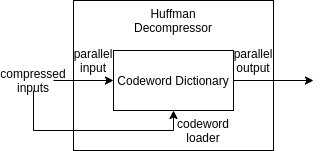
\includegraphics[scale=1]{Huffman Decompressor Block Diagram.png}
	\caption{Huffman Decompressor Block Diagram}
	\label{fig:huffman_decompressor_block_diagram}
\end{figure}

The decompressor is much simpler than the compressor. First, the decompressor reads the plaintext tree data in from thread 0. In the plaintext tree, each character has a static bit width, and all possible characters in the Huffman tree are always transmitted, even if there are fewer characters than that used. The data is always transmitted unencoded character first, followed by the static-length character encoding, followed by the length of the encoding. Once this data is processed for each character, decompression can begin.

With the tree stored in the dictionary, the decompressor then decodes each configured thread separately. If a matched codeword is the escape codeword, the decompressor reads out the bits after the escape word to get the literal character being referred to. Otherwise, the decompressor reads the correct value from the dictionary. This continues until every thread has decoded the correct number of characters.

% TODO: for components that aren't in standard LZ77, give an example of the inputs to that module and what the outputs would be
% TODO: for components that are already in standard LZ77, reference when they happen in the examples given in the Background section
\section{LZ77}\label{se:lz77}
\subsection{High-Level Design Choices}\label{se:lz77_design_choices}
This section of the paper describes the high-level design of each of the compressors and decompressors, the modifications to the algorithms used, and the motivations for the changes. Information about the low-level implementation details of the design is included in a later section.

\subsubsection{Compressor}\label{sss:lz77_compressor_design}
The LZ77 compressor and decompressor hardware mostly implements its algorithm unchanged. As with the other designs, it is fully parameterized, and the design parameters and typical values can be found in \ref{tab:lz77-configuration-table}. The major difference between this LZ77 implementation and the normal LZ77 algorithm is that this implementation always selects the first, longest CAM match, and can only match up to `CAM max pattern length` characters in the CAM.

\begin{table}[htb]
	\centering
	\caption{Configurable LZ77 Parameters and their typical values.}
	\begin{tabular}{cc}
	    \toprule
	    Parameter & Typical Value \\
	    \midrule
	    Character bits & 8 \\
	    \midrule
	    CAM characters & 4096 \\
	    \midrule
	    CAM max pattern length & 16 \\
	    \midrule
	    Max pattern length & 266 \\ 
	    \midrule
	    Escape character & 103 \\ 
	    \midrule
	    Decompressor max characters out & 8\\
	    \bottomrule
	\end{tabular}
	\label{tab:lz77-configuration-table}
\end{table}

The LZ77 compressor reads each byte into a buffer of size `CAM max pattern length`. Once this buffer is full, the pattern is searched in a CAM which returns the longest, first occurrence and the length of the occurrence. If the length of the occurrence is less than `CAM max pattern length` but equal to or greater than the number of bytes needed to encode a pattern, the CAM outputs a pattern instead of the literal bytes. If the length is the maximum, then the state of the state machine changes, and each byte after the pattern is checked against the input bytes. This continues until the bytes no longer match or the length reaches `Max pattern length`. Otherwise, the first character in the buffer is output as a literal character, and the pattern buffer shifts in a new value from the input.

Compressed data always follows the same format. First, the escape character value appears, then a bit that is negated from the most significant bit of the escape character, then the pointer to where in the CAM the data is, then the length of the data. If the length of the data exceeds the value that can be shown by one character of `Character bits` width, then another character of the same width is added to the encoding after that, until the `Max pattern length` is reached or this is terminated by a value that is less than the maximum possible value. However, this means that escape characters cannot be encoded properly, so two escape characters in a row encodes a single literal value of the escape character. The negated escape character bit in the encoded data format ensures that encoded data is not mistaken for two escape characters in a row.

The above information about the encoding for patterns does not make any assumptions on the size of a character or the size of a pattern. This is because the design does not either. The design can be generated for any configuration, and the encoding of patterns in the design will be adjusted to reflect the configuration.

\subsubsection{Decompressor}\label{sss:lz77_decompressor_design}
The decompressor for the LZ77 hardware, like the other decompressors, is much simpler than the compressor. It reads in multiple bytes at a time, and if the first byte is a literal, it outputs a single byte corresponding to that literal. If the input is a pattern encoding, the decompressor transitions to a state where it outputs `Decompressor max characters out` characters from the history every cycle until it has exhausted all characters in the pattern, then goes back to reading the initial state, ready to read more data.

\subsection{Implementation Details}\label{se:lz77_implementation_details}
This section of the paper describes the low-level implementation details of each of the compressors and decompressors and the reasoning for those implementations.

\subsubsection{Compressor}\label{sss:lz77_compressor_implementation}

\begin{figure}[htb]
	\centering
	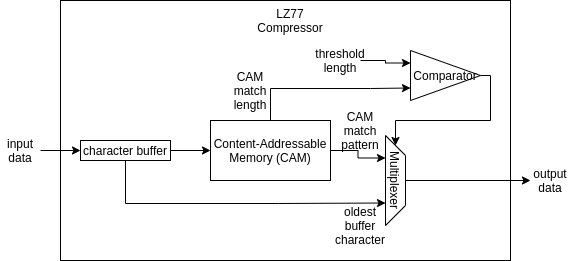
\includegraphics[scale=0.8]{LZ77 Compressor.png}
	\caption{LZ77 Compressor Block Diagram}
	\label{fig:lz77_compressor_block_diagram}
\end{figure}

The LZ77 compressor consists of two primary components: a pattern search module that uses a CAM to search for multi-character patterns in the byte history combinationally, and the state machine and logic that utilize the pattern search module to perform LZ77 compression.

% TODO: hardware doesn't output wires, it has wires that it outputs values on
% TODO: add a sentence describing not just the functional level, what the inputs and outputs of the CAM do, but HOW it calculates those things
The pattern search module uses an internal multi-character CAM. This CAM can receive data to be written and can receive patterns of data to search. The CAM outputs multiple large arrays of wires, with each array representing the matches of one of the characters in the search data. Each wire in the array is a boolean value representing whether or not the character at that position in the CAM is a match for the character being compared against. Additionally, the CAM provides an output that gives access to all of its stored data so that, when matches longer than `CAM max pattern length` are found, the state machine of the LZ77 compressor can check their true length.

The pattern search module uses the output of the internal CAM to find patterns up to length `CAM max pattern length`. It does this by submitting a pattern to the CAM, then left-shifting each boolean array of matches from the CAM by its index and performing a bitwise AND between them. As each aditional array AND is performed, the remaining true values in the array correspond to the starting indices of patterns that match a number of characters. Once all ANDs have been performed, the only remaining true values in the array are the indices of the starting points for patterns that matched the CAM input entirely. By reversing the resulting arrays of wires and using the Chisel3 lastIndexWhere() function, the first matching index of patterns of each length can be found. The results of each of these lastIndexWhere() functions can be chosen by performing an AND reduction on each resulting array of wires in the bitwise AND operation previously described, and picking the longest pattern that returns a true value from this reduction.

The state machine that controls compression stores the input data in a buffer. The buffer must be filled, and then each clock cycle, the buffer is checked against the pattern search module. If a pattern is of a length such that the number of characters to encode the pattern is less than or equal to the number of characters in the pattern, the pattern is compressed. Otherwise, the oldest character in the buffer is shifted out while a new character is shifted in, the old character is added to the byte history, and the old character is output as a literal character.

When a pattern is long enough to be compressed, the encoding starts off with an escape character determined by the `escape character` parameter. If the escape character is a literal representation of that character value, the escape character occurs twice in a row. If not, the escape character is followed by the negation of the most significant bit in the escape character, then the starting index of the pattern in the byte history, then the number of characters in the pattern. This encoding is character-aligned, which causes it to work very well with Huffman encoding. However, to keep the encoding character-aligned while allowing long patterns, the encoding can have a variable length. The smallest length of the encoding occurs when the number of characters in the pattern can be added into the remaining bits after the escape character, negation bit, and index are all used. Because a pattern always has a minimum length, the pattern's length is always incremented by the pattern's break-even length to increase the efficiency of the encoding. If the pattern is too long to be represented this way, the maximum length value is set, and the next character's value is added to the pattern length. This can continue arbitrarily until the maximum number of characters in a pattern is reached. 

\subsubsection{Decompressor}\label{sss:lz77_decompressor_implementation}

\begin{figure}[htb]
	\centering
	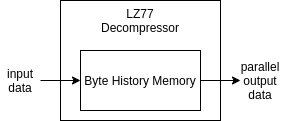
\includegraphics[scale=1]{LZ77 Decompressor.png}
	\caption{LZ77 Decompressor Block Diagram}
	\label{fig:lz77_decompressor_block_diagram}
\end{figure}

The LZ77 decompressor takes enough characters to allow the largest possible pattern encoding from the LZ77 compressor to be read in a single cycle. If the first character in the input data is not an escape character or is two escape characters in a row, it is counted as a literal that is output and added to the character history. Otherwise, a state machine is used to read bytes from the character history in parallel. The LZ77 decompressor continues to take inputs until the configured number of bytes is decompressed, then finishes.

\section{LZW}\label{ss:lzw}
This section discusses the LZW compressor and decompressor. First, it introduces the high-level design choices of this hardware, then it describes the details of the implementation.

\subsection{High-Level Design Choices}\label{se:high-level_design_choices}
This section of the paper describes the high-level design of each of the compressors and decompressors, the modifications to the algorithms used, and the motivations for the changes. Information about the low-level implementation details of the design is included in a later section.

\subsubsection{Compressor}\label{sss:lzw_compressor_design}
The LZW compressor and decompressor are very close to functioning exactly like LZW. Like the other designs, the LZW compressor and decompressor are fully parameterized. Parameters and their typical values are listed in \ref{tab:lzw-configuration-table}. The LZW compressor streams in one character per cycle and adds it into a buffer to match against existing patterns in the dictionary. Once a pattern no longer matches anything in the dictionary, the last pattern match is sent to the output, and all but the last byte of the pattern are shifted out of the pattern buffer. The pattern buffer is built up again, repeating this cycle until there are no more characters to be compressed.

\begin{table}[htb]
	\centering
	\caption{Configurable LZW Parameters and their typical values.}
	\begin{tabular}{cc}
	    \toprule
	    Parameter & Typical Value \\
	    \midrule
	    character bits & 8 \\
	    \midrule
	    maximum characters in a sequence & 16 \\
	    \midrule
	    maximum elements in the dictionary & 768 \\ 
	    \midrule
	    enable debugging statistics & false \\
	    \bottomrule
	\end{tabular}
	\label{tab:lzw-configuration-table}
\end{table}

The only differences compared to a software LZW implementation are limitations of hardware: there is a limit to the size of the pattern buffer and to the number of entries in the dictionary. If the dictionary is full of patterns, no new patterns will be added, but the hardware can continue to compress as normal. And if a pattern fills the entire pattern buffer, further instances of it will not continue to be added to the dictionary. Other than that, the LZW hardware compressor is normal.

\subsubsection{Decompressor}\label{sss:lzw_decompressor_design}
The decompressor is even simpler than the compressor. Every time it reads an input, it outputs the resulting dictionary entry, and adds a new item to the dictionary based on the last pattern and the first byte of the current pattern. Like the compressor, it only avoids adding an element to the dictionary if the dictionary is full or the pattern is already as long as it can become.

\subsection{Implementation Details}\label{se:lzw_implementation_details}
This section of the paper describes the low-level implementation details of each of the compressors and decompressors and the reasoning for those implementations.

% TODO: for components that aren't in standard LZW, give an example of the inputs to that module and what the outputs would be
% TODO: for components that are already in standard LZW, reference when they happen in the examples given in the Background section
\subsubsection{Compressor}\label{sss:lzw_compressor_implementation}

\begin{figure}[htb]
	\centering
	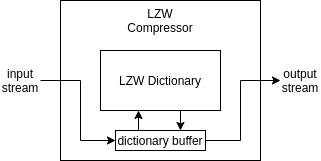
\includegraphics[scale=1]{LZW Compressor.png}
	\caption{LZW Compressor Block Diagram}
	\label{fig:lzw_compressor_block_diagram}
\end{figure}

The LZW compressor requires fewer steps to work than the Huffman compressor, so it is implemented in a single monolithic module. The most important part of the LZW compressor design is the dictionary. Each entry in the dictionary can hold a number of values equal to `maximum characters in a sequence` Additionally, each entry in the dictionary stores the number of character values it holds. The dictionary starts with a list of each literal character where the character's index in the dictionary is equal to its encoded value and its length is one character.

The LZW compressor reads in characters one-at-a-time to a character buffer. The size of this buffer is determined by the `maximum characters in a sequence` parameter. Each time a new character is added to the buffer, the character is checked against the existing LZW dictionary and the length of matching entries is checked to be sure any matches are valid. Every match is held until the next clock cycle, and once the buffer is full or there is no match in the dictionary, the last match is output and the buffer is cleared. If a match was output because the buffer was full, the buffer is completely emptied, and if not, the buffer is emptied except for the most recently added character. Every time the buffer is cleared because there was no existing match, a new entry is added to the dictionary representing the character sequence in the buffer.

When an output is transmitted, the LZW compressor also sends the number of bits of the data, so the wrapping module is able to pack the output values correctly. As the LZW dictionary grows, the number of bits required to represent an index in the dictionary grows as well.

This sequence of filling and emptying the buffer and adding characters to the dictionary is repeated until there are no more remaining characters. If there are no more remaining characters but there is still data left in the character buffer, the `stop` signal can be asserted to force the compressor to output a match corresponding to the data still held in the character buffer.

\subsubsection{Decompressor}\label{sss:lzw_decompressor_implementation}

\begin{figure}[htb]
	\centering
	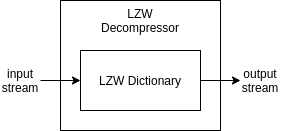
\includegraphics[scale=1]{LZW Decompressor.png}
	\caption{LZW Decompressor Block Diagram}
	\label{fig:lzw_decompressor_block_diagram}
\end{figure}

The LZW decompressor works in much the same way as the compressor, minus the character buffer. The decompressor also starts with the dictionary containing an entry for each literal character. Each of these entries still have a character length of one, and the index of each entry still matches its character value. The LZW decompressor takes outputs from the compressor and uses them as indices to look up sequences in the dictionary. It outputs each of the sequences in parallel. It also outputs the number of bits each input index currently consists of so that the hardware sending the data can correctly increment whatever counters are being used to send the unaligned data, because the number of bits in an input changes as the size of the dictionary increases.

For each sequence that is not the maximum length, it and the first character of the following sequence are added to the dictionary. This makes sure that the LZW decompressor's dictionary stays in sync with the dictionary of the compressor. Unlike the LZW compressor, there is no need for a stop signal to send the final bytes of data, so once the input data is exhausted, all the output data will be transmitted as well.

\chapter{Methodology} \label{ch:methodology}
This chapter discusses the methodology that was used to generate data about the designs in this work. It also contains details about the ways existing designs can be compared to this work.

\section{Hardware Synthesis}\label{se:hardware_synthesis}
All designs were implemented with the ASAP7 7nm Predictive PDK with the Synopsys Design Compiler. First, designs were synthesized with a target clock period of 10 picoseconds. The synthesis tools will fail to meet this unreasonable expectation, but the negative slack from this synthesis run can be used to find the fastest possible clock speed and the area usage of the design at this speed. A second run at the correct maximum clock speed can then be used to find power information, if desired.

\section{IBM Area Estimation}\label{se:ibm_area_estimation}
Unfortunately, in \cite{ibm}, IBM does not provide exact area numbers for the compression and decompression acceleration engine. However, \cite{wikichip-ibm-area} has a die photograph and area estimation for a POWER9 CPU. Using this and the claim that the acceleration engine took up less than 0.5\% of the entire chip's area, the area of the acceleration engine can be approximated. 

\section{Compression Ratio Comparison}\label{se:compression_ratio_comparison_methodology}
To compare memory compression ratios of the hardware designs with existing software implementations, memory dumps were taken randomly during benchmarks from SPEC, Sparkbench, Parsec, and other benchmarks. These memory dumps were then parsed into 4 KB pages of memory. These pages were randomly sampled and compressed and decompressed with Gzip (which uses Deflate), and the hardware designs from this work. Although no hardware Deflate compressor or decompressor exists as part of this work, the pages were also compressed and decompressed with LZ77 and Huffman sequentially to demonstrate the difference between software and hardware implementations of the same algorithm.

The goal of this compression ratio comparison was to determine how much effective RAM could be achieved with memory compression using each design. Because of this, all pages that compressed to larger than 4 KB were treated as being exactly 4 KB for the average compression ratio calculation, as an incompressible page would remain in an uncompressed form during normal OS memory compression.

\section{Latency}\label{se:latency}
To calculate software compression latency, Gzip was timed compressing several thousand 4 KB memory dump pages in a row, then the time was divided by the number of pages. This was done because a single compression often occurs too quickly to accurately time, so multiple sequential compression operations were needed.

For hardware latency calculations, the latency can be found by multiplying the fastest possible clock period of each design with the number of cycles required to complete compression or decompression with the design. 

\chapter{Results and Analyses} \label{ch:results}
This chapter delivers the results of the investigations detailed in Chapter \ref{ch:methodology} and analyzes them.

\section{ASIC Area and Frequency Comparison}\label{se:asic_area_and_frequency_comparison}
Figure \ref{fig:maximum_clock_speeds} shows the highest clock speeds achievable by each design configuration. As can be seen, most of the designs are capable of achieving at least 2 GHz, except for the LZ77 compressor and the LZW decompressor. The reason for the LZ77 compressor's lower than expected clock speed is not currently known. Initial investigations into the clock speed by dividing the design up and synthesizing it as separate pieces suggest that the reduction in clock speed is not due to the CAM or pattern search module, so must be due to the state machine. However, the state machine does not contain much additional logic, so it is currently unclear what components cause the slowdown.

As for the LZW decompressor, although its hardware is simpler than the LZW compressor, the compressor takes two cycles per byte compressed. The LZW decompressor only uses one cycle per input pattern. It seems that the synthesis tools are able to perform register retiming on the LZW compressor to make it faster, but that this retiming is not possible on the decompressor because fewer cycles are available for each additional pattern to the dictionary. This also must be investigated further to be determined certainly.

The authors of \cite{ibm} do not discuss the specifics of the clock speeds attainable by the hardware. However, they mention that the target clock speeds are 2.0-2.5 GHz. The IBM POWER9 and z15 compressors are implemented on a 14 nm manufacturing node. Although there is no way to make a direct comparison between the GlobalFoundries node used by IBM and the ASAP7 PDK, \cite{wikichip-manufacturing-conversion} provides a way to approximate. If it is assumed that the difference between the GlobalFoundries 14 nm node and ASAP7 is the same as the difference between TSMC's 16 nm node and TSMC's 7 nm node described in \cite{wikichip-manufacturing-conversion}, then IBM would be able to achieve speeds 35-40\% faster than the POWER9 compression engine, meaning it would be in the range of 2.7-3.5 GHz. This would mean that its clock speeds are faster than most of the designs of this work. However, it is important to note that \cite{ibm} is heavily optimized to achieve these clock speeds, and the most important aspect of the design is not clock frequency, but total memory latency.

\begin{figure}[htb]
	\centering
	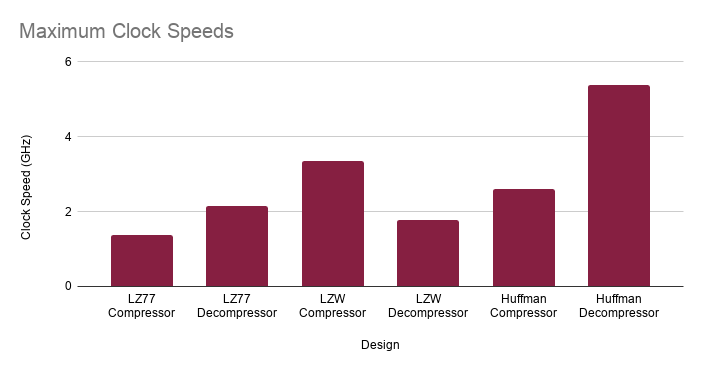
\includegraphics[scale=0.6]{Maximum Clock Speeds.png}
	\caption{Maximum Clock Speeds}
	\label{fig:maximum_clock_speeds}
\end{figure}

Although not all of the designs can achieve similar clock speeds to the IBM compression accelerator, they are certainly much more configurable due to their parameterization. As can be seen from Figure \ref{fig:design_configuration_area_comparison}, all of the areas of the designs in this work can be significantly changed based on the configuration. The compressor and decompressor with the largest capability for change, LZW, can change in size more than an order of magnitude, depending on what values the parameters are set to.

The designs in this work also achieve much lower areas than the IBM work. Figure \ref{fig:synthesized_area_results} shows the area results of the design configurations chosen to be compared to the IBM implementation. Although IBM does not publish the exact area of the POWER9 compression engine, \cite{ibm} mentions that the compression engine takes less than 0.5\% of the total chip area. Additionally, estimates of the die area from photographs can be used to indicate the approximate area of the IBM design\cite{wikichip-ibm-area}. For a direct comparison to the IBM area estimate, Figure \ref{fig:synthesized_area_results} shows the area of the designs from this work and IBM, normalized to the smallest design in this work. As is evident, the smallest design in this work is 866x smaller than IBM's accelerator, and even the largest design in this work is still 18.6x smaller than IBM's design. 

\begin{figure}[htb]
	\centering
	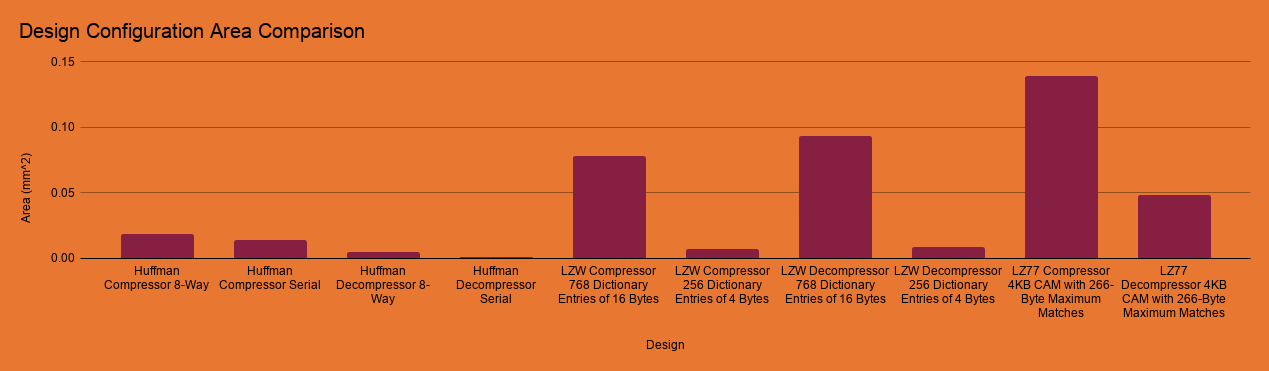
\includegraphics[scale=0.29]{Design Configuration Area Comparison.png}
	\caption{Design Configuration Area Comparison}
	\label{fig:design_configuration_area_comparison}
\end{figure}
\begin{figure}[htb]
	\centering
	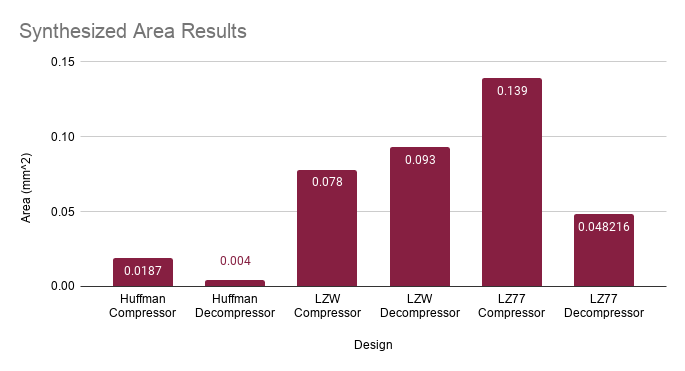
\includegraphics[scale=0.6]{Synthesized Area Results.png}
	\caption{Synthesized Area Results}
	\label{fig:synthesized_area_results}
\end{figure}
\begin{figure}[htb]
	\centering
	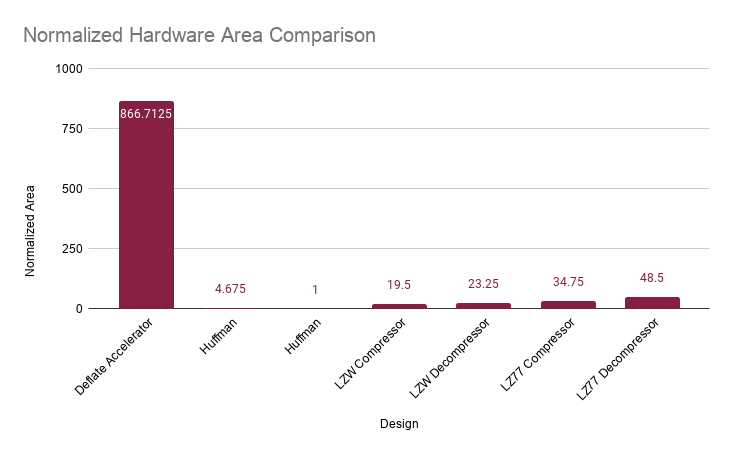
\includegraphics[scale=0.6]{Normalized Hardware Area Comparison.png}
	\caption{Normalized Hardware Area Comparison}
	\label{fig:normalized_hardware_area_comparison}
\end{figure}

% TODO: Add clock cycle counters to each of the compressors and decompressors to get the accurate latency. Even if some of the hardware can't do this, provide numbers for the hardware that can. I think this can be done by adding big Chisel Queues at the outputs of the compressors that can store all the compressor outputs, then only starting the decompressors after the compressors are done.
\section{Latency Comparison}\label{se:latency_comparison}
To compare latencies to the IBM design, first it is important to calculate the latencies of the IBM design. For the purposes of comparing against this work's designs, it is most fair to compare IBM's latency to compress or decompress a 4 KB page of memory. The IBM paper states, `We model the accelerator execution time \emph{T} with $T=T_{0}+Data\_Size/PeakBandwidth$ where constant \emph{$T_{0}$} is the setup time with is the software and hardware initialization delays before the accelerator starts processing data.` \cite{ibm}. To get the overall hardware latency of the IBM design, the hardware latency portion of \emph{$T_{0}$} needs to be known, and the result of $Data\_Size/PeakBandwidth$ needs to be known for compression and decompression. The sum of these will be the hardware latency for IBM's implementations.

The hardware latency portion of \emph{$T_{0}$} can be found without difficulty. Later in the paper, Abali et. al state, `Therefore, with multithreading software delays nearly disappear in the total delay calculations and the 8-thread latencies in Table II reveal the actual NXU hardware latencies in the 0.55-0.73\emph{$\mu$} range` \cite{ibm}. The table referred to can then be used to find the hardware latency for compression and decompression for both the z15 and POWER9 accelerator engines.

The latency once the hardware is initialized requires some additional math, but can be found from IBM's description as well. The IBM paper says that, `When the data size is $Half\_Peak\_Data\_Size=T_{0} \times PeakBandwidth$ we get $T=2T_{0}$, which means that half the time is spent in the setup and the other half in the accelerator doing actual processing.` \cite{ibm}. From this, we can deduce that $PeakBandwidth=Half\_Peak\_Data\_Size \div T_{0}$. The peak data size of 4 KB is already known, so the final equation for this portion of the latency is $4KB/(Half\_Peak\_Data\_Size \div T_{0})$. These remaining variables can both be found in the IBM paper's Table II, so it is possible to calculate the hardware latency of each accelerator. The latency of each accelerator is shown in Table \ref{tab:ibm_latencies}.

\begin{table}[htb]
	\centering
	\caption{Hardware Latencies of IBM Compression and Decompression Accelerators}
	\begin{tabular}{cc}
	    \toprule
	    Hardware Design & Total Hardware Latency ($\mu$s) \\
		\midrule
		POWER9 Compressor & 1.1 \\
		\midrule
		z15 Compressor & 0.88 \\
		\midrule
		POWER9 Decompressor & 1.21 \\
		\midrule
		z15 Decompressor & 1.205 \\
		\bottomrule
	\end{tabular}
	\label{tab:ibm_latencies}
\end{table}

Because I have all of the necessary information for my designs, it is much simpler to calculate the total latencies. The minimum and maximum compression and decompression latencies are simply the most and fewest possible cycles to compress or decompress a page multiplied by the clock period of a single cycle.

Figure \ref{fig:compression_design_latencies} and Figure \ref{fig:decompression_design_latencies} show the latency comparison between the IBM accelerator and this work. As can be seen in these graphs, the minimum decompression latencies from the designs in this work have significantly lower decompression latencies than the IBM designs. However, although the designs in this work demonstrate significantly improved decompression latencies, it is important to note that the compression latencies are often higher with the designs from this work, and the Deflate hardware design is hypothetical.

The maximum decompression latencies are significantly faster for my design than the IBM design, but these maximum decompression latencies can only be reached when the data is completely incompressible. If data is incompressible, then there is no need for it to be stored in memory in a compressed form, so no need for it to be decompressed. In all cases with reasonable compression ratios for the compressed memory, the latency of my hardware designs is significantly better than the maximum decompression latency, moving the performance of this design closer to an order of magnitude lower than IBM's.

The compression latencies are often higher with my designs. However, this is not as much of a concern with memory compression as the decompression latencies. This is because, while the decompression is on the critical path to completing computations, the compression latency is not. Once a compression operation has been submitted, the CPU could move on while the memory write was buffered and compressed in the background.

The final note on these figures is that the Deflate hardware design shown is hypothetical. The latency numbers for this design make the conservative assumption that no pipelining can take place between LZ77 and Huffman compression or decompression, and each stage completes separately before the next one starts. Even making this assumption, my hardware designs could achieve significantly lower latencies than IBM if they were combined to form a Deflate compressor and decompressor.

\begin{figure}[htb]
	\centering
	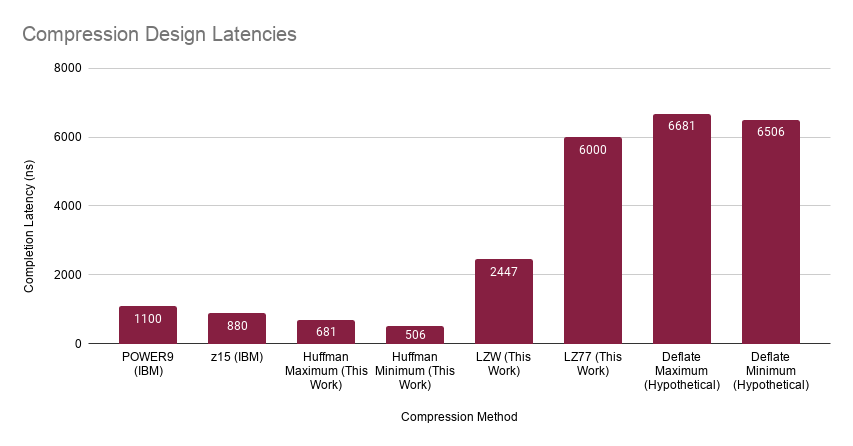
\includegraphics[scale=0.5]{Compression Design Latencies.png}
	\caption{Compression Design Latencies}
	\label{fig:compression_design_latencies}
\end{figure}
\begin{figure}[htb]
	\centering
	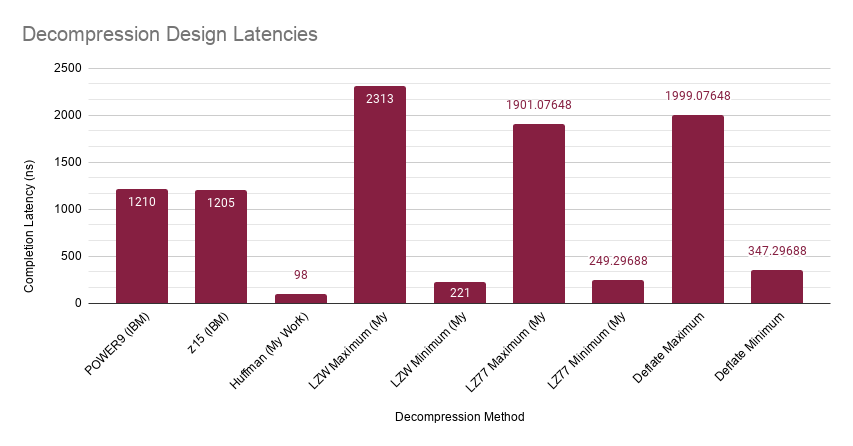
\includegraphics[scale=0.5]{Decompression Design Latencies.png}
	\caption{Decompression Design Latencies}
	\label{fig:decompression_design_latencies}
\end{figure}

% TODO: Look to see if IBM has their data corpus used available so we could download it and try it with our hardware. It looks like they used Silesia, Canterbury, and Calgary.
\section{Compression Ratio Comparison}\label{se:compression_ratio_comparison_results}
Although decompression latency is very important, it must not be at the cost of significant data compressibility. If the memory compressibility is significantly reduced, then there is no point to compressing the memory in the first place. Figure \ref{fig:benchmark_memory_dump_compressibility} shows the compression ratios achieved by each of the hardware designs as configured above. Additionally, LZ77+Huffman on the graph shows the performance of a hypothetical design combining LZ77 compression and Huffman decompression to create a Deflate compressor. This figure shows that on average, the LZ77+Huffman hardware is capable of achieving compression ratios 87\% as high as the software Deflate implementation. While this reduction is non-negligible, it is not enough to completely negate the value of memory compression, and the latency reduction of several orders of magnitude is likely worth the slightly reduced compressibility. This is especially true in the context of operating system memory compression. Because the operating system often does not compress memory data to a byte granularity, it is quite possible that many workloads would see similar or identical effective memory from the hardware implementation and the software implementation.

\begin{figure}[htb]
	\centering
	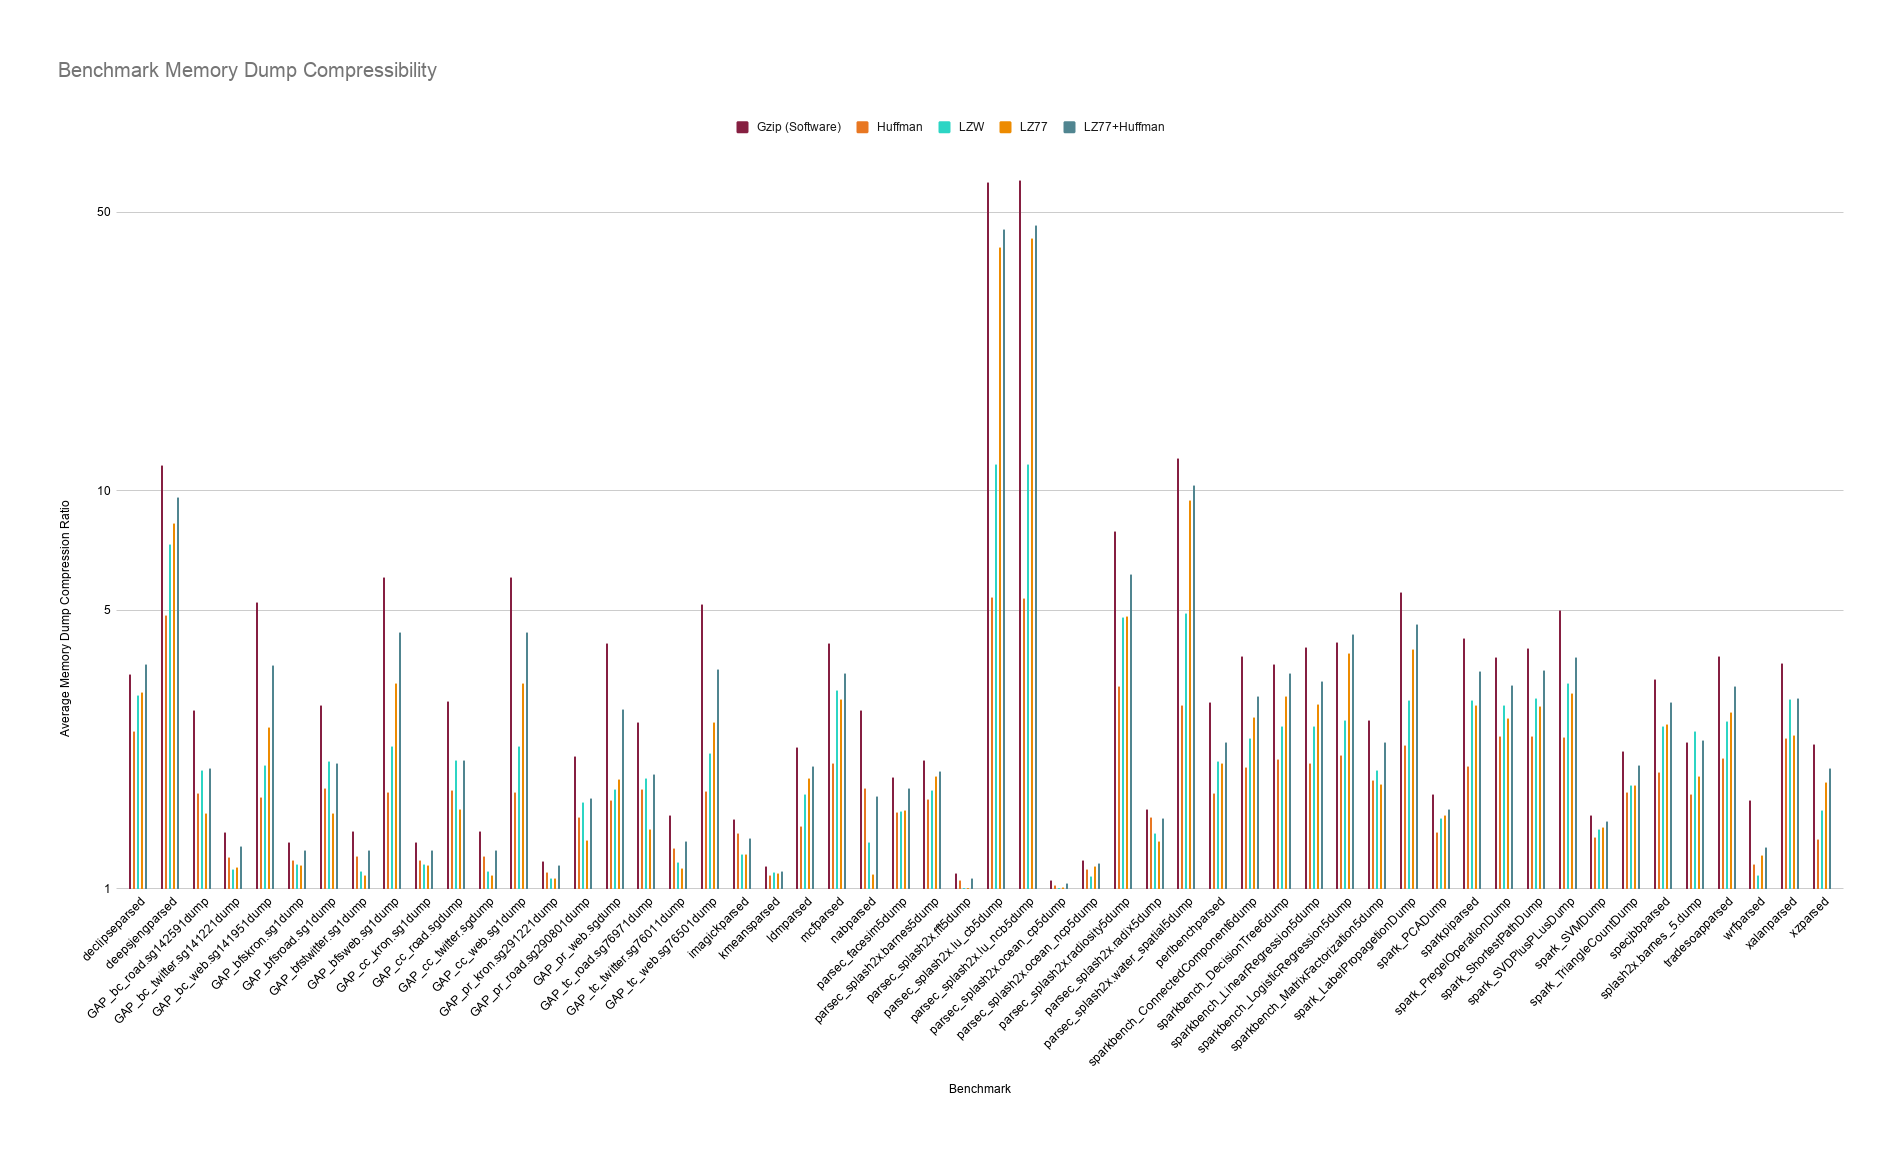
\includegraphics[scale=0.357]{Benchmark Memory Dump Compressibility.png}
	\caption{Benchmark Memory Dump Compressibility}
	\label{fig:benchmark_memory_dump_compressibility}
\end{figure}

\chapter{Limitations and Future Work} \label{ch:discussion}
Although this works compares very well to the current state of the art, there are a number of potential improvements that could strengthen it significantly. In this chapter, these potential improvements will be discussed in order of potential benefit.

Currently, the LZ77 decompressor design is capable of decompressing multiple characters per cycle when given an encoded pattern. However, when the LZ77 decompressor receives uncompressed literal characters, it currently processes them one-at-a-time, sequentially. This makes the LZ77 decompression latency very closely tied to the compressibility of the data. To fix this, it would be we could support multiple bytes of literal input per cycle. A naive implementation would only do this search if there were no escape characters at all in the characters read in parallel. However, a more complex implementation could support variable parallel read speeds, only reading characters that come before an escape character in the input data. This would significantly decouple the decompression latency from the compressibility of the data, improving the speed of nearly all decompression operations by a significant margin.

The designs would also benefit from being formally verified. Although the designs have each been tested with over 400,000 4 KB memory dump files without any bugs found, it is possible that there are edge cases that have not been reached that could cause the hardware designs to compress or decompress incorrectly. Formal verification is a method of mathematically proving that a design has certain characteristics, given a set of initial assumptions. If the designs were formally verified to never incorrectly compress or decompress data, this would make them significantly better candidates for incorporating into an ASIC. Additionally, an easy-to-use formal verification flow would allow for faster design changes, because bugs could be caught as soon as they were written and tested.

While the designs are all able to achieve low latencies, some of the designs are not able to run above 2 GHz. Because one of the ideal use cases of these designs are in a memory controller, it would be good for the designs to be able to run at the clock speeds common in server CPUs, somewhere in the 2-3 GHz range. This would allow integration into memory controllers without the need for multiple clock domains. Additionally, if this could be achieved without increasing the number of cycles needed to perform the compression or decompression operations, increasing the clock speeds of the designs would also further reduce latency.

Another valuable future work would be to add the design to a larger project. Currently, the designs have only been tested in an isolated context. Adding the designs to something like a memory controller or FPGA to accelerate compression and decompression would provide valuable feedback about how easily the design can be interfaced with. This is an important future work, as it is the motivation for open-sourcing this work.

While this work is primarily targeted towards memory compression with its low latencies, all of the designs in this work have very low area overhead. Additionally, they implement algorithms that are frequently used for data outside of memory compression. While it has not yet been investigated, it would be interesting to see the compression ratios and performance that could be expected from these designs in a file or network compression context.  It seems likely that they would perform well, but it is yet to be seen.

It would also be interesting if the physical design and tool flow was fully open-source. The software used for synthesis, Synopsys Design Compiler, is expensive and proprietary. To match the open-source nature of this project and the other tools used by it, it would be interesting to see the physical design aspects fully open-sourced as well. The OpenROAD project seems to have made significant headway into an open-source, fully-automated RTL-to-GDS toolflow \cite{openroad}. It would be interesting to see this work implemented in all of the currently supported manufacturing nodes on OpenROAD or another similar open-source project. In this way, every possible aspect of the design and tooling could be open-source and free for anyone to try.

Finally, it would be beneficial to create software libraries that are compatible with the compressors and decompressors shown in this work. Many previous works utilize only a compression accelerator or only a decompression accelerator \cite{hardwarelz4, fpgahuffmanlz77, gziponachip, hdfsgzip, ribeiro, deflatedecompression, lzrw1}. However, because modifications have been made to all of the algorithms used in this work, there do not currently exist any software implementations that are compatible with the hardware.  To further improve the flexibility of the design, it would be valuable to implement performant, configurable software implementations of the compressors and decompressors.

% TODO: Dr. Cameron says probably at least another page needed here. Discuss broader implications, what can we do now that we couldn't previously, who can benefit, what can people do with this, give examples and numbers
\chapter{Conclusions} \label{ch:conclusions}
As workloads continue to eat up more RAM, memory compression will continue to become an important cost-saving tool. Although the existing compression accelerators are able to significantly reduce the latency of compression and decompression, existing accelerators are several times slower than an uncompressed memory access. This work improves upon the existing state of the art by reducing the decompression latency by over an order of magnitude and 33\% in the best case and worst case, respectively. Additionally, this work does so while reducing the area by over an order of magnitude. Most importantly, this work is open-source under the MIT license, so it is available for future research groups to continue to improve upon and modify. If it is used, it has the potential to save researchers hundreds or thousands of hours of work re-implementing the same compression algorithms in hardware.

% This is the standard bibtex file. Do not include the .bib extension in <bib_file_name>.
% Uncomment the following lines to include your bibliography: 
\bibliography{related_works}
\bibliographystyle{plainnat}   

	% This formats the chapter name to appendix to properly define the headers:
% 	\appendix

	% Add your appendices here. You must leave the appendices enclosed in the appendices environment in order for the table of contents to be correct.
% 	\begin{appendices}
% 		\chapter{First Appendix} \label{app:appendix_one}
% 			\section{Section one} \label{ase:app_one_sect_1}
% 			\section{Section two} \label{ase:app_one_sect_2}
% 		\chapter{Second Appendix} \label{app:appendix_two}
% 	\end{appendices}

\end{document}


%****************************************************************************
% Below are some general suggestions for writing your dissertation:
%
% 1. Label everything with a meaningful prefix so that you
%    can refer back to sections, tables, figures, equations, etc.
%    Usage \label{<prefix>:<label_name>} where some suggested
%    prefixes are:
%			ch: Chapter
%     		se: Section
%     		ss: Subsection
%     		sss: Sub-subsection
%			app: Appendix
%     		ase: Appendix section
%     		tab: Tables
%     		fig: Figures
%     		sfig: Sub-figures
%     		eq: Equations
%
% 2. The VTthesis class provides for natbib citations. You should upload
%	 one or more *.bib bibtex files. Suppose you have two bib files: some_refs.bib and 
%    other_refs.bib.  Then your bibliography line to include them
%    will be:
%      \bibliography{some_refs, other_refs}
%    where multiple files are separated by commas. In the body of 
%    your work, you can cite your references using natbib citations.
%    Examples:
%      Citation                     Output
%      -------------------------------------------------------
%      \cite{doe_title_2016}        [18]
%      \citet{doe_title_2016}       Doe et al. [18]
%      \citet*{doe_title_2016}      Doe, Jones, and Smith [18]
%
%    For a complete list of options, see
%      https://www.ctan.org/pkg/natbib?lang=en
%
% 3. Here is a sample table. Notice that the caption is centered at the top. Also
%    notice that we use booktabs formatting. You should not use vertical lines
%    in your tables.
% 
%				\begin{table}[htb]
%					\centering
%					\caption{Approximate computation times in hh:mm:ss for full order 						versus reduced order models.}
%					\begin{tabular}{ccc}
%						\toprule
%						& \multicolumn{2}{c}{Computation Time}\\
%						\cmidrule(r){2-3}
%						$\overline{U}_{in}$ m/s & Full Model & ROM \\
%						\midrule
%						0.90 & 2:00:00 & 2:08:00\\
%						0.88 & 2:00:00 & 0:00:03\\
%						0.92 & 2:00:00 & 0:00:03\\
%						\midrule
%						Total & 6:00:00 & 2:08:06\\
%						\bottomrule
%					\end{tabular}
%					\label{tab:time_rom}
%				\end{table}
% 
% 4. Below are some sample figures. Notice the caption is centered below the
%    figure.
%    a. Single centered figure:
%					\begin{figure}[htb]
%						\centering
%						\includegraphics[scale=0.5]{my_figure.eps}
%						\caption{Average outlet velocity magnitude given an average  
%				        input velocity magnitude of 0.88 m/s.} 
%						\label{fig:output_rom}
%					\end{figure}
%    b. Two by two grid of figures with subcaptions
%					\begin{figure}[htb]
%						\centering
%						\begin{subfigure}[h]{0.45\textwidth}
%							\centering
%							\includegraphics[scale=0.4]{figure_1_1.eps}
%							\caption{Subcaption number one}
%							\label{sfig:first_subfig}
%						\end{subfigure}
%						\begin{subfigure}[h]{0.45\textwidth}
%							\centering
%							\includegraphics[scale=0.4]{figure_1_2.png}
%							\caption{Subcaption number two}
%							\label{sfig:second_subfig}
%						\end{subfigure}
%
%						\begin{subfigure}[h]{0.45\textwidth}
%							\centering
%							\includegraphics[scale=0.4]{figure_2_1.pdf}
%							\caption{Subcaption number three}
%							\label{sfig:third_subfig}
%						\end{subfigure}
%						\begin{subfigure}[h]{0.45\textwidth}
%							\centering
%							\includegraphics[scale=0.4]{figure_2_2.eps}
%							\caption{Subcaption number four}
%							\label{sfig:fourth_subfig}
%						\end{subfigure}
%						\caption{Here is my main caption describing the relationship between the 4 subimages}
%						\label{fig:main_figure}
%					\end{figure}
%
%----------------------------------------------------------------------------
%
% The following is a list of definitions and packages provided by VTthesis:
%
% A. The following packages are provided by the VTthesis class:
%      amsmath, amsthm, amssymb, enumerate, natbib, hyperref, graphicx, 
%      tikz (with shapes and arrows libraries), caption, subcaption,
%      listings, verbatim
%
% B. The following theorem environments are defined by VTthesis:
%      theorem, proposition, lemma, corollary, conjecture
% 
% C. The following definition environments are defined by VTthesis:
%      definition, example, remark, algorithm
%
%----------------------------------------------------------------------------
%
%  I hope this template file and the VTthesis class will keep you from having 
%  to worry about the formatting and allow you to focus on the actual writing.
%  Good luck, and happy writing.
%    Alan Lattimer, VT, 2016
%
%****************************************************************************





